
\chapter{线丛、到射影空间的映射与除子}
\label{ch:line-bundles-divisors}

初次学习\trAlgebraicGeometry{}时，听说\trLineBundle（\trInvertibleSheaf）竟如此性命攸关，会让人惊讶。i)~它们当然是最简单的\trVectorBundle。ii)~我们常常能借助「\trCodimension{} $1$」的信息把它们分类。特别地，我们可以构造它们、操控它们。iii)~知道\trVariety{} $X$ 上的\trLineBundle，有助于我们分类 $X$、理解到\trProjectiveSpace{}与到其他\trVariety{}的映射。iv)~而这只是个开头。

本章接下来描述研究\trLineBundle{}并对之分类的方便而有力的办法。我们从一个基本的例子——\trProjectiveSpace{}上的线丛 $\OO(m)$——开始（\S15.1）。然后讨论\trLineBundle{}连同一些\trSection{}如何给出到\trProjectiveSpace{}的映射，以及到射影概形的映射如何全都以这种方式产生（\S15.2）。这同时是初等的、精妙的、有力的。在 \S15.3 中，我们描述「到\trProjectiveSpace{}的单参数族有唯一极限」这一观念的一个具体化。接下来是本章最具挑战性的部分（\S15.4）：我们引入 \trWeil{}除子，并在若干情形下用它们定出 $X$ 上的全部\trLineBundle。辛苦的付出带来许多可以亲手算出的有趣例子（\S15.5）。随后我们讨论把某些\trLineBundle{}轻易描述为恰好可逆的理想层的一条不同途径（\trEffectiveCartierDivisor，\S15.6）。我们以再度沟通射影概形上\trQCSheaf{}与分次模的一节收尾（\S15.7）。


\section{射影空间上的一些线丛}

我们现在来描述\trField{} $k$ 上的\trProjectiveSpace{}中一族重要的\trInvertibleSheaf。

作为热身，我们从 $\mathbb{P}^1_k=\Proj k[x_0,x_1]$ 上的\trInvertibleSheaf{} $\OO_{\mathbb{P}^1_k}(1)$ 开始。下标 $\mathbb{P}^1_k$ 指明的是该\trSheaf{}所栖身的空间，当上下文已足够清楚时，它常被省去。我们用\trTransitionFunction{}来描述\trInvertibleSheaf{} $\OO(1)$。它在通常的\trAffine\trOpenSet{} $U_0=\mathrm{D}(x_0)=\Spec k[x_{1/0}]$ 与 $U_1=\mathrm{D}(x_1)=\Spec k[x_{0/1}]$ 上是\trTrivial{}的。（我们继续沿用 $x_{i/j}$ 这一约定来描述\trProjectiveSpace{}各小块上的坐标；见 \S4.4.9。）于是，$U_0$ 上一个\trSection{}的数据就是 $x_{1/0}$ 的一个多项式。从 $U_0$ 到 $U_1$ 的\trTransitionFunction{}是乘以 $x_{0/1}=x_{1/0}^{-1}$。而从 $U_1$ 到 $U_0$ 的\trTransitionFunction{}于是便是乘以 $x_{1/0}=x_{0/1}^{-1}$。

这一信息总结如下：
\begin{center}
\begin{tikzcd}[column sep=4.5em, row sep=3.2em]
\text{\trOpenCover} & U_0=\Spec k[x_{1/0}] & U_1=\Spec k[x_{0/1}] \\
\text{\trTrivialization{}与\trTransitionFunction} & k[x_{1/0}] \ar[r, bend left=14, "\times x_{0/1}=x_{1/0}^{-1}"] & k[x_{0/1}] \ar[l, bend left=14, "\times x_{1/0}=x_{0/1}^{-1}"']
\end{tikzcd}
\end{center}

为检验我们的理解，让我们来算一算 $\OO(1)$ 的\trGlobalSections。这将推广我们亲手做过的那个计算 $\Gamma(\mathbb{P}^1_k,\OO_{\mathbb{P}^1_k})\cong k$（\mbox{例~4.4.6}）。一个整体截面就是一个多项式 $f(x_{1/0})\in k[x_{1/0}]$ 连同一个多项式 $g(x_{0/1})\in k[x_{0/1}]$，使得 $f(1/x_{0/1})x_{0/1}=g(x_{0/1})$。稍加思索便会发现，$f$ 必为线性：$f(x_{1/0})=ax_{1/0}+b$，从而 $g(x_{0/1})=a+bx_{0/1}$。于是
\[
\dim\Gamma(\mathbb{P}^1_k,\OO(1))=2\ne 1=\dim\Gamma(\mathbb{P}^1_k,\OO).
\]
于是，$\OO(1)$ 并不同构于 $\OO$——我们构造出了第一个（得到证明的）非平凡\trLineBundle{}例子！

我们接下来更一般地定义 $\mathbb{P}^1_k$ 上的 $\OO_{\mathbb{P}^1_k}(m)$。其定义方式与前完全相同，只是诸\trTransitionFunction{}取为 $\OO(1)$ 的那些\trTransitionFunction{}的 $m$ 次幂。
\begin{center}
\begin{tikzcd}[column sep=4.5em, row sep=3.2em]
\text{\trOpenCover} & U_0=\Spec k[x_{1/0}] & U_1=\Spec k[x_{0/1}] \\
\text{\trTrivialization{}与\trTransitionFunction} & k[x_{1/0}] \ar[r, bend left=14, "\times x_{0/1}^m=x_{1/0}^{-m}"] & k[x_{0/1}] \ar[l, bend left=14, "\times x_{1/0}^m=x_{0/1}^{-m}"']
\end{tikzcd}
\end{center}

特别地，多亏这些显式的\trTransitionFunction，我们看到 $\OO(m)=\OO(1)^{\otimes m}$（若 $m$ 为负，其含义也是显然的：$(\OO(1)^{\otimes(-m)})^{\vee}$）。同样显然地还有 $\OO(m)\otimes\OO(m')=\OO(m+m')$。

\textbf{15.1.A.（重要练习）}\quad 证明：当 $m\ge 0$ 时 $\dim\Gamma(\mathbb{P}^1,\OO(m))=m+1$，否则为 $0$。

\textbf{15.1.1.}\ \emph{\trhExample{}。}\quad 很久以前（在\cref{ex:ox-module-tensor-product}(a) 中），我们曾警告过：对 $\OO_X$-\trModule{}作张量时需要\trSheafification——若 $\mathscr{F}$ 与 $\mathscr{G}$ 是某个\trRingedSpace{}上的两个 $\OO_X$-\trModule，那么 $\mathscr{F}(X)\otimes_{\OO_X(X)}\mathscr{G}(X)\cong(\mathscr{F}\otimes\mathscr{G})(X)$ 未必成立。如今我们便有了一个例子：令 $X=\mathbb{P}^1_k$、$\mathscr{F}=\OO(1)$、$\mathscr{G}=\OO(-1)$，并利用 $\OO(-1)$ 没有非零整体截面这一事实。

\textbf{15.1.B.（练习）}\quad 证明：若 $m\ne m'$，则 $\OO(m)\ncong\OO(m')$。由此推得：我们有群的单射 $\mathbb{Z}\hookrightarrow\operatorname{Pic}\mathbb{P}^1_k$，由 $m\mapsto\OO(m)$ 给出。

把 $\OO(m)$ 的\trGlobalSections{}等同于 $x_0$、$x_1$ 的次数为 $m$ 的\trHomogeneous{}多项式——也就是说，等同于 $k[x_0,x_1]$ 的次数 $m$ 部分——是很有用的（向 $\mathbb{P}^n$ 的推广见 \S15.1.2）。你能从\mbox{练习~15.1.A}的解答中看出这一点吗？我们将会看到，这一等同在许多方面都是\trNatural{}的。比如说，你可以证明 $\OO(m)$ 的定义不依赖于\trAffine\trCover{}的选取，而这个多项式描述同样不依赖于覆盖。（为此，见\mbox{例~4.5.13}；日后你可以把它与\mbox{练习~25.1.N}相比较。）作为对这一观点之有用性的一个立竿见影的检验，问问你自己：$\OO(3)$ 的\trSection{} $x_0^3-x_0x_1^2$ 在何处消失？$\OO(1)$ 的\trSection{} $x_0+x_1$ 可以乘上 $\OO(2)$ 的\trSection{} $x_0^2$，得到 $\OO(3)$ 的一个\trSection。是哪一个？$\OO(-2)$ 的有理\trSection{} $x_0^4(x_1+x_0)/x_1^7$ 在何处有\trZeros、在何处有\trPole，阶数各是多少？（\trZeros{}与\trPole{}的概念我们曾在\mbox{定义~13.5.7}见过，日后还将在 \S15.4 中与它们重逢；但你凭直觉此刻便应能回答这些问题。）

现在我们在\trProjectiveSpace{} $\mathbb{P}^n_k$ 上定义\trInvertibleSheaf{} $\OO_{\mathbb{P}^n_k}(m)$。在通常的\trAffine\trOpenSet{} $U_i=\Spec k[x_{0/i},\dots,x_{n/i}]/(x_{i/i}-1)=\Spec A_i$ 上，它是\trTrivial{}的，于是诸\trSection{}（作为 $A_i$-\trModule）同构于 $A_i$。从 $U_i$ 到 $U_j$ 的\trTransitionFunction{}是乘以 $x_{i/j}^m=x_{j/i}^{-m}$。
\begin{center}
\begin{tikzcd}[column sep=3.4em, row sep=3.2em]
U_i=\Spec k[x_{0/i},\dots,x_{n/i}]/(x_{i/i}-1) & U_j=\Spec k[x_{0/j},\dots,x_{n/j}]/(x_{j/j}-1) \\
k[x_{0/i},\dots,x_{n/i}]/(x_{i/i}-1) \ar[r, bend left=14, "\times x_{i/j}^m=x_{j/i}^{-m}"] & k[x_{0/j},\dots,x_{n/j}]/(x_{j/j}-1) \ar[l, bend left=14, "\times x_{j/i}^m=x_{i/j}^{-m}"']
\end{tikzcd}
\end{center}
请注意：这些\trTransitionFunction{}显然满足\trCocycleCondition。

\textbf{15.1.C.（必要练习；参看\mbox{练习~9.3.J}、\mbox{定理~18.1.2}）}\quad 证明：$\dim_k\Gamma(\mathbb{P}^n_k,\OO_{\mathbb{P}^n_k}(m))=\binom{n+m}{n}$。

\textbf{15.1.2.}\quad 如同 $\mathbb{P}^1$ 的情形，$\mathbb{P}^n_k$ 上 $\OO(m)$ 的诸\trSection{}会被\trNatural{}地等同于我们这 $n+1$ 个变元的次数为 $m$ 的\trHomogeneous{}多项式。（这一与\trHomogeneous{}多项式的联系将在下一道练习中被置于更精确的立足点上。）于是 $x+y+2z$ 是 $\mathbb{P}^2$ 上 $\OO(1)$ 的一个\trSection。它不是一个函数，但我们知道这个\trSection{}在哪里消失——恰好就在 $x+y+2z=0$ 之处。

此外，请注意：对固定的 $n$，$\binom{n+m}{n}$ 是变元 $m$ 的一个 $n$ 次多项式，但只在 $m\ge 0$ 时如此（更好的说法：当 $m\ge -n$ 时）。这应当是在向你暗示：这个函数「想当一个多项式」，但若无襄助便不会成功。我们日后将定义 $h^0(\mathbb{P}^n_k,\OO(m)):=\dim_k\Gamma(\mathbb{P}^n_k,\OO(m))$，再往后我们还将定义更高次的上同调群，并且我们将定义 \emph{欧拉示性数}（Euler characteristic）$\chi(\mathbb{P}^n_k,\OO(m)):=\sum_{i=0}^{\infty}(-1)^i h^i(\mathbb{P}^n_k,\OO(m))$（上同调在高于 $n$ 的次数上都将消失）。我们将会发现这样一条道理：欧拉示性数比 $h^0$ 表现得更规矩，因此我们现在就应当怀疑（并在日后证明；见\mbox{定理~18.1.2}、\mbox{注记~18.3.5}与\mbox{练习~18.3.C}）：这个多项式其实就是欧拉示性数，而它之所以在 $m\ge 0$ 时与 $h^0$ 相合，是因为其余的上同调群全都消失。

最后我们指出：对任意的\trRing{} $A$，我们都可以在 $\mathbb{P}^n_A$ 上定义 $\OO(m)$：上述定义原封不动地适用，而且\mbox{练习~15.1.C}立即推广，表明 $\Gamma(\mathbb{P}^n_A,\OO_{\mathbb{P}^n_A}(m))$ 是一个秩为 $\binom{n+m}{n}$ 的自由 $A$-\trModule，并且可以用\trHomogeneous{}多项式作出同样的解读。

\textbf{15.1.D.（练习；发人深省的例子，也是好的锻炼）}\quad 设 $n>0$。设 $\pi\colon\mathbb{A}^{n+1}_A\setminus V(x_0,\dots,x_n)\to\mathbb{P}^n_A$ 是态射 $(x_0,\dots,x_n)\mapsto[x_0,\dots,x_n]$（描述见练习~7.3.F 与例~7.3.12）。对任意 $m\in\mathbb{Z}$，描述一个同构
\[
\pi^*\OO_{\mathbb{P}^n_A}(m)\overset{\sim}{\longleftrightarrow}\OO_{\mathbb{A}^{n+1}_A\setminus V(x_0,\dots,x_n)}.
\]
这诱导出一个映射 $\pi^*\colon\Gamma(\mathbb{P}^n_A,\OO_{\mathbb{P}^n_A}(m))\to\Gamma(\mathbb{A}^{n+1}_A\setminus V(x_0,\dots,x_n),\OO_{\mathbb{A}^{n+1}_A})$。证明（如 \S4.4.1 中那样）：拉回
\[
\alpha\colon A[x_0,\dots,x_n]=\Gamma(\mathbb{A}^{n+1}_A,\OO_{\mathbb{A}^{n+1}_A})\longrightarrow\Gamma(\mathbb{A}^{n+1}_A\setminus V(x_0,\dots,x_n),\OO_{\mathbb{A}^{n+1}_A})
\]
是一个同构，并解释复合
\[
\alpha^{-1}\circ\pi^*\colon\Gamma(\mathbb{P}^n_A,\OO_{\mathbb{P}^n_A}(m))\longrightarrow A[x_0,\dots,x_n]
\]
如何把 $\Gamma(\mathbb{P}^n_A,\OO_{\mathbb{P}^n_A}(m))$ 解读为 $A[x_0,\dots,x_n]$ 中次数为 $m$ 的\trHomogeneous{}多项式。

\textbf{15.1.3.\ 这些是 $\mathbb{P}^n_k$ 上仅有的\trLineBundle。}

设 $k$ 是一个\trField。我们将在 \S15.4.15 中见到：这些 $\OO(m)$ 正是 $\mathbb{P}^n_k$ 上仅有的\trInvertibleSheaf。下一道练习便在 $n=1$ 时证明了这一点。

\textbf{15.1.E.（练习）}\quad 证明：$\mathbb{P}^1_k$ 上的每个\trInvertibleSheaf{}都形如 $\OO(m)$，其中 $m$ 为某个整数。提示：利用主理想整环上\trFinitelyGenerated{}\trModule{}的分类（\mbox{注记~6.4.4}）来证明 $\mathbb{A}^1_k$ 上的一切\trInvertibleSheaf{}都是\trTrivial{}的（\mbox{练习~14.2.C} 的特例）。然后把问题归结为确定 $\mathbb{P}^1_k$ 的标准覆盖中那两个\trOpenSubset{}之间可能的\trTransitionFunction。

警示：$\mathbb{P}^1_A$ 上可以存在不具 $\OO(m)$ 形式的\trInvertibleSheaf。日后你或许能想出例子。（为你懂得更多之时备下的寻例提示：若 $\Spec A$ 不连通会怎样？抑或，若那引出的例子傻得可以，那么若 $\Spec A$ 带有非平凡的\trInvertibleSheaf{}又会怎样？）

\textbf{15.1.4.\ 射影 $A$-\trScheme{}上的\trLineBundle。}

设 $M_\bullet$ 是一个分次 $S_\bullet$-\trModule。定义\trGradedModule{} $M(m)_\bullet$ 如下：$M(m)_d:=M_{m+d}$。于是，\trQCSheaf{} $\widetilde{M(m)_\bullet}$ 满足
\[
\Gamma(\mathrm{D}_+(\mathrm{f}),\widetilde{M(m)_\bullet})=((M_\bullet)_f)_m,
\]
这里的下标意指我们取的是次数 $m$ 的分次分片。（无可否认，这些下标容易让人犯晕！）

\textbf{15.1.F.（练习）}\quad 若 $S_\bullet=A[x_0,\dots,x_n]$，从而 $\Proj S_\bullet=\mathbb{P}^n_A$，证明 $\widetilde{S(m)_\bullet}\cong\OO(m)$，此时要用到\trTransitionFunction（参看 \S15.1）。（回想\mbox{练习~15.1.D}：$\OO(m)$ 的诸\trGlobalSections{}应当等同于 $x_0,\dots,x_n$ 中次数为 $m$ 的\trHomogeneous{}多项式。你能在本题的情境中看出这一点吗？）

\textbf{15.1.5.}\ \emph{\trhDefinition{}。}\quad 受此启发，若 $S_\bullet$ 是一个在次数 $1$ 处生成的\trGradedRing，我们便定义 $\OO_{\Proj S_\bullet}(m)$（或简单地记作 $\OO(m)$，此时 $S_\bullet$ 是隐含的）为 $\widetilde{S(m)_\bullet}$。

\textbf{15.1.G.（重要练习）}\quad 若 $S_\bullet$ 在次数 $1$ 处生成，证明 $\OO_{\Proj S_\bullet}(m)$ 是一个\trInvertibleSheaf。

若 $S_\bullet$ 在次数 $1$ 处生成，而 $\mathscr{F}$ 是 $\Proj S_\bullet$ 上的一个\trQCSheaf，则定义 $\mathscr{F}(m):=\mathscr{F}\otimes\OO(m)$。这常称为\textbf{用 $\OO(m)$ 扭转 $\mathscr{F}$}，或\textbf{用 $m$ 扭转 $\mathscr{F}$}。更一般地，若 $\mathscr{L}$ 是一个\trInvertibleSheaf，则 $\mathscr{F}\otimes\mathscr{L}$ 常称为\textbf{用 $\mathscr{L}$ 扭转 $\mathscr{F}$}。

\textbf{15.1.H.（练习）}\quad 若 $S_\bullet$ 在次数 $1$ 处生成，证明 $\widetilde{M_\bullet}(m)\cong\widetilde{M(m)_\bullet}$。（此后，在这类情形里，我们对那个「点」摆在何处便可以满不在乎了。）

\textbf{15.1.I.（练习）}\quad 若 $S_\bullet$ 在次数 $1$ 处生成，证明 $\OO(m_1+m_2)\cong\OO(m_1)\otimes\OO(m_2)$。

\textbf{15.1.6.}\ \hard\ \emph{不重要的注记。}\quad 即便 $S_\bullet$ 不在次数 $1$ 处生成，那么（若 $S_\bullet$ 是\trFinitelyGenerated{}的）由\mbox{练习~7.4.G}，对某个 $d$，$S_{d\bullet}$ 便在次数 $1$ 处生成。此时我们可以定义\trInvertibleSheaf{} $\OO(dm)$，其中 $m\in\mathbb{Z}$。这并\emph{不}意味着我们\emph{不能}定义 $\OO(1)$；这取决于 $S_\bullet$。例如，若 $S_\bullet$ 是\trPolynomialRing{} $k[x,y]$，带有通常的分次、只是去掉了诸一次项（于是 $S_\bullet=k[x^2,xy,y^2,x^3,x^2y,xy^2,y^3]$），那么 $S_{2\bullet}$ 与 $S_{3\bullet}$ 都在次数 $1$ 处生成，也就是说我们可以定义 $\OO(2)$ 与 $\OO(3)$。有充分的理由把二者的「差」称作 $\OO(1)$。（这套代数或许会让你想起\trPinchedPlane，见\mbox{练习~13.5.H}。\footnote{原书此处作（may remind of you of），当系「remind you of」之误，径改。——译者注}）



\section{线丛与到射影空间的映射}

回想一下，\trAffine{}空间 $\mathbb{A}^n$ 曾有一个作为\trRepresentableFunctor{}的简短描述：映入 $\mathbb{A}^n$ 的（从 $X$ 出发的）映射，恰与「在 $X$ 上选取 $n$ 个函数」这份数据完全相同（\mbox{练习~7.6.E}(a)）。在本节中，我们会不经意间把\trProjectiveSpace{}也按同样的方式重新解释一遍。

设 $x_0$、$x_1$、$x_2$ 是 $\mathbb{P}^2_k$ 上的射影坐标。你能看出
\begin{equation*}\tag{15.2.0.1}\label{eq:cubic-map-morphism}
[x_0^3,\; x_0^2x_2,\; x_0x_1x_2+x_1^3,\; x_2^3]
\end{equation*}
如何给出一个\trMorphism{} $\mathbb{P}^2_k\to\mathbb{P}^3_k$ 吗？\eqref{eq:cubic-map-morphism} 的各个分量并不是函数，所以我们无法逐个地理解它们。但对 $\mathbb{P}^2_k$ 的任何一个「点」，它们的比值仍可以有意义。例如，点 $[1,1,1]$ 被送到 $[1,1,2,1]$，而同一个点 $[2,2,2]$ 被送到 $[8,8,16,8]$，所以这里并无矛盾——\eqref{eq:cubic-map-morphism} 的各个分量都是 $3$ 次\trHomogeneous{}的，因此一个分量除以另一个分量所得的\trQuotient{}是一个\trRationalFunction。反过来看，
\begin{equation*}\tag{15.2.0.2}\label{eq:cubic-map-failed}
[x_0^3,\; x_0^2x_2,\; x_0x_1x_2+x_1^3,\; x_1^3]
\end{equation*}
并不给出一个\trMorphism{} $\mathbb{P}^2_k\to\mathbb{P}^3_k$，因为点 $[0,0,1]$「不知道自己该去哪里」。但你或许能够把 \eqref{eq:cubic-map-failed} 解读为给出一个\trMorphism{} $\mathbb{P}^2_k\setminus\{[0,0,1]\}\to\mathbb{P}^3_k$，或者一个\trRationalMap{} $\mathbb{P}^2_k\dashrightarrow\mathbb{P}^3_k$。这甚至可能让你想起\mbox{练习~7.3.O}。现在我们就把这件事精确化，并且以笼统得多的方式陈述之。特别地，我们将不需要在\trField{}上工作。

\textbf{15.2.A.（容易的练习：一个性命攸关的重要构造）}\quad 设 $s_0,\dots,s_n$ 是某个\trScheme{} $X$ 上一个\trInvertibleSheaf{} $\mathscr{L}$ 的 $n+1$ 个\trGlobalSections，没有公共\trZeros。定义一个相应的到 $\mathbb{P}^n$ 的映射：
\[
X\xrightarrow{\;[s_0,\dots,s_n]\;}\mathbb{P}^n.
\]
提示：若 $U$ 是其上 $\mathscr{L}$ 为\trTrivial{}的一个\trOpenSubset，则选取一个\trTrivialization，用这个\trTrivialization{}把诸 $s_i$ 翻译成函数，并用\mbox{练习~7.3.O}(a) 得到一个\trMorphism{} $U\to\mathbb{P}^n$。然后利用\mbox{练习~7.3.O}(b) 证明：所有这些映射（对不同的 $U$ 与不同的\trTrivialization）都相互「相合」。

（在\mbox{定理~15.2.2} 中我们将会看到：这给出的是到\trProjectiveSpace{}的\emph{一切}映射。）注意，这道练习按其书写原样「在 $\mathbb{Z}$ 上工作」（因为一切\trMorphism{}都「在」\trScheme{}的\trCategory{}的\trFinalObject{}「之上」），尽管许多读者只会在某个\trField{} $k$ 上工作。

\textbf{15.2.1.}\ \emph{\trhDefinition{}。}\quad 若 $\mathscr{L}$ 是 $X$ 上的一个\trInvertibleSheaf，则 $\mathscr{L}$ 的一切\trGlobalSections{}都消失的那些点称为 $\mathscr{L}$ 的\textbf{\trBasePoint}（base points），而\trBasePoint{}组成的集合称为 $\mathscr{L}$ 的\textbf{\trBaseLocus}（base locus）；它是 $X$ 的一个\trClosedSubset。（我们可以把它精细化成一个\trClosedSubscheme：取 $\mathscr{L}$ 的诸\trSection{}的消失\trLocus{}的\trSchemeTheoretic{}交，便得到\textbf{\trSchemeTheoretic{}\trBaseLocus}（scheme-theoretic base locus）。）\trBaseLocus{}的补集是\textbf{\trBasePointFree\trLocus}（base-point-free locus）。若 $\mathscr{L}$ 没有\trBasePoint，则称它是\textbf{\trBasePointFree}的（base-point-free）。\trBasePointFree\trLocus{}是 $X$ 的一个\trOpenSubset。

更一般地，若我们有 $\mathscr{L}$ 的一批\trGlobalSections（未必是全部），则可以定义这些\trSection{}的\trBasePoint（以及上一段中所有相关的观念）。于是，例如，\mbox{练习~15.2.A} 陈述的是：若 $s_0,\dots,s_n$ 是 $X$ 上一个\trInvertibleSheaf{} $\mathscr{L}$ 的\trBasePointFree{}的\trGlobalSections{}族，则它们定义了一个到 $\mathbb{P}^n$ 的映射。

$k$-\trScheme{} $X$ 上的一个\textbf{\trLinearSystem}（linear series）（或\textbf{线性系}（linear system））是一个 $k$-\trVectorSpace{} $V$（通常是\trFiniteDimensional{}的）、一个\trInvertibleSheaf{} $\mathscr{L}$，以及一个线性映射 $\lambda\colon V\to\Gamma(X,\mathscr{L})$。这样的\trLinearSystem{}常被径称作「$V$」，其余数据隐含不写。若映射 $\lambda$ 是一个\trIsomorphism，则称它为\textbf{完全\trLinearSystem}（complete linear series），且常记作 $|\mathscr{L}|$。\trBasePoint{}的语言（\trBasePointFree、\trBaseLocus、\trSchemeTheoretic{}\trBaseLocus、……）可以径直施用于\trLinearSystem{}（\trBasePointFree\trLinearSystem、……）。

作为一项现实检验，\mbox{练习~15.2.A} 陈述的是：$k$-\trScheme{} $X$ 上一个 $(n+1)$ 维的\trLinearSystem，连同基的一个选取，设其\trBasePointFree\trLocus{}为 $U$，便定义了一个\trMorphism{} $U\to\mathbb{P}^n_k$。

\textbf{15.2.B.（容易的练习）}\quad 若 $\mathscr{L}$ 与 $\mathscr{M}$ 都是\trBasePointFree{}的\trInvertibleSheaf，证明 $\mathscr{L}\otimes\mathscr{M}$ 亦然。

\textbf{15.2.C.（练习）}\quad 设我们有一个\trMorphism{} $\pi\colon X\to\mathbb{P}^n_k$，对应于\trBasePointFree\trLinearSystem \allowbreak$\Gamma(\mathbb{P}^n_k,\OO(1))\to\Gamma(X,\mathscr{L})$（于是 $\mathscr{L}=\pi^*\OO(1)$）。若 $X$ 在 $\mathbb{P}^n_k$ 中的\trSchemeTheoreticImage{}落于一张\trHyperplane{}之中，我们便说这个\trLinearSystem（或 $X$ 本身）是\textbf{\trDegenerate}（degenerate）的（否则称\textbf{非\trDegenerate}（nondegenerate）的）。证明：一个\trBasePointFree\trLinearSystem $V\to\Gamma(X,\mathscr{L})$ 是非\trDegenerate{}的，当且仅当映射 $V\to\Gamma(X,\mathscr{L})$ 是一个\trInclusionMap。特别地，完全\trLinearSystem{}总是非\trDegenerate{}的。

\mbox{定理~15.2.2}——\mbox{练习~15.2.A} 的逆命题，或者说其补全——将给出\trLineBundle{}之所以至关紧要的一个理由：它们向我们讲述到\trProjectiveSpace{}的映射，乃至更一般地，到\trQuasiprojective{} $A$-\trScheme{}的映射。鉴于我们给任何非\trQuasiprojective{}的\trScheme{}起名字一直起得很费劲，它们实际上是向我们讲述着到实质上一切有意思的\trScheme{}的映射。

\textbf{15.2.2.\ 重要定理。}\ ——\ \emph{对固定的\trScheme{} $X$，\trMorphism{} $X\to\mathbb{P}^n$ 与数据 $(\mathscr{L},s_0,\dots,s_n)$ 成\trBijection，其中 $\mathscr{L}$ 是一个\trInvertibleSheaf，而 $s_0,\dots,s_n$ 是 $\mathscr{L}$ 的没有公共\trZeros{}的\trSection{}（也就是说，$(s_0,\dots,s_n)$ 是\trBasePointFree{}的），且在相差这些数据的\trIsomorphism{}的意义下视作相同。}

（这在 $\mathbb{Z}$ 上、乃至任意的\trBaseScheme{}上都行得通。）非正式地说：到 $\mathbb{P}^n$ 的\trMorphism{}对应于一个\trLineBundle{}的 $n+1$ 个\trSection，它们不在任何一点处全部消失，再模去 $\OO_X^\times$ 的\trGlobalSections，因为乘以一个可逆函数给出 $\mathscr{L}$ 的一个\trAutomorphism。这是代数几何中那样一类要紧的定理之一：证明容易，但其效果对于人们应当如何思考而言却相当微妙。要恰当地消化它需要一些时间。一个「\trCoordinateFree」的版本见\mbox{练习~15.2.G}。

\textbf{15.2.3.}\quad \mbox{定理~15.2.2} 描述了到\trProjectiveSpace{}的一切\trMorphism，因此按照\trYoneda{}哲学，这可以被取作\trProjectiveSpace{}的一个\emph{定义}：它在相差唯一\trIsomorphism{}的意义下确定\trProjectiveSpace。\emph{\trProjectiveSpace{} $\mathbb{P}^n$（在 $\mathbb{Z}$ 上）是\trLineBundle{} $\mathscr{L}$ 连同 $n+1$ 个无公共\trZeros{}的 $\mathscr{L}$-\trSection{}的\trModuliSpace。}（你能给出一个在 $X$ 上、记作 $\mathbb{P}^n_X$ 的\trProjectiveSpace{}的类似定义吗？）或者，如果你愿意，$k$-\trScheme{}之间的映射 $X\to\mathbb{P}^n$ 对应于 $X$ 上的 $(n+1)$ 维\trBasePointFree\trLinearSystem，连同基的选取。（若把 $k$ 换成另一个\trRing，你会如何改述这句话？）

每当你看到一个到\trProjectiveSpace{}的映射时，你应当立刻同时在头脑中保有着那个\trInvertibleSheaf{}与那些\trSection{}（或者，如果你愿意，那个\trLinearSystem）。

到射影概形的映射可以类似地描述。例如，若 $Y\hookrightarrow\mathbb{P}^2_k$ 是\trCurve{} $x_2^2x_0=x_1^3-x_1x_0^2$，则从一个\trScheme{} $X$ 到 $Y$ 的映射由 $X$ 上一个\trInvertibleSheaf{}连同三个无公共\trZeros{}的\trSection{} $s_0$、$s_1$、$s_2$ 给出，且满足 $s_2^2s_0-s_1^3+s_1s_0^2=0$。

\textbf{15.2.4.}\quad \mbox{定理~15.2.2} 之证明的中心想法是直截了当的：我们需要展示一个\trBijection，所以只消弄清楚从左到右与从右到左的映射各是什么，并证明二者确实互逆。关键将在于思考诸\trTrivialization{}邻域之间的\trTransitionFunction。

更精确地说，\mbox{定理~15.2.2} 的对应如下。任意 $n+1$ 个无公共\trZeros{}的 $\mathscr{L}$-\trSection{}确定一个到 $\mathbb{P}^n$ 的\trMorphism{}，靠的是\mbox{练习~15.2.A}。反之，若你有一个到\trProjectiveSpace{}的映射 $\pi\colon X\to\mathbb{P}^n$，那么我们有 $\OO_{\mathbb{P}^n}(1)$ 的 $n+1$ 个\trSection，对应于那些超平面截面，即 $x_0,\dots,x_n$。于是 $\pi^*x_0,\dots,\pi^*x_n$ 是 $\pi^*\OO_{\mathbb{P}^n}(1)$ 的\trSection，并且它们没有公共\trZeros{}。（提醒：把拉回\trInvertibleSheaf{}想成拉回\trTransitionFunction，是很有帮助的。）

于是为了证明\mbox{定理~15.2.2}，我们只需要证明这两个构造无论按哪个方向复合都给出恒等。

\emph{重要定理~15.2.2 的证明。}\quad 设给定一个\trInvertibleSheaf{} $\mathscr{L}$ 的 $n+1$ 个无公共\trZeros{}的\trSection{} $s_0,\dots,s_n$，它们（经由\mbox{练习~15.2.A}）诱导一个\trMorphism{} $\pi\colon X\to\mathbb{P}^n$\footnote{原书此句作（induced from $(s_1,\dots,s_n)$ and $\pi$），其中 $(s_1,\dots,s_n)$ 当系 $(s_0,\dots,s_n)$ 之误（该态射由全组截面诱导），径改。——译者注}。对每个 $s_i$，我们在 $s_i$ 不消失的开集 $X_{s_i}$ 上得到 $\mathscr{L}$ 的一个\trTrivialization。$\mathscr{L}$ 的诸\trTransitionFunction{}在 $X_{s_i}\cap X_{s_j}$ 上恰好就是 $s_i/s_j$。由于 $\OO(1)$ 在 $\mathbb{P}^n$ 的标准\trAffine\trOpenSet{} $\mathrm{D}_+(x_i)$ 上是\trTrivial{}的，$\pi^*(\OO(1))$ 在 $X_{s_i}=\pi^{-1}(\mathrm{D}_+(x_i))$ 上是\trTrivial{}的。此外，$s_i/s_j=\pi^*(x_{i/x_j})$（径直得自\mbox{练习~15.2.A} 中 $\pi$ 的构造）。这就给出了一个\trIsomorphism{} $\mathscr{L}\overset{\sim}{\hookrightarrow}\pi^*\OO(1)$——这两个\trInvertibleSheaf{}有着相同的\trTransitionFunction。

\textbf{15.2.D.（练习）}\quad 证明：这个\trIsomorphism{}可以被选得使得
\[
(\mathscr{L},s_0,\dots,s_n)\overset{\sim}{\longleftrightarrow}(\pi^*\OO(1),\pi^*x_0,\dots,\pi^*x_n),
\]
从而补全该定理两个方向的蕴含之一。

对另一个方向，设给定一个映射 $\pi\colon X\to\mathbb{P}^n$。令 $s_i=\pi^*x_i\in\Gamma(X,\pi^*(\OO(1)))$。由于诸 $x_i$ 在 $\mathbb{P}^n$ 上没有公共\trZeros，诸 $s_i$ 在 $X$ 上没有公共\trZeros。映射 $[s_0,\dots,s_n]$ 与映射 $\pi$ 相同。我们如下看出这一点。$\mathrm{D}(x_i)$（在\trMorphism{} $[s_0,\dots,s_n]$ 之下）的原像是 $\mathrm{D}(s_i)=\mathrm{D}(\pi^*x_i)=\pi^{-1}\mathrm{D}(x_i)$，于是「右边的开集跑到右边的开集」。为了证明两个\trMorphism{} $\mathrm{D}(s_i)\to\mathrm{D}(x_i)$（分别由 $(s_0,\dots,s_n)$ 与 $\pi$ 诱导）相同，我们利用这样一个事实：到一个\trAffineScheme{} $\mathrm{D}(x_i)$ 的映射由其反方向的\trGlobalSections{}映射所确定（\mbox{必作练习~7.3.G}）。两个\trMorphism{} $\mathrm{D}(s_i)\to\mathrm{D}(x_i)$ 都对应于\trRingMorphism{} $\pi^{\sharp}\colon x_{j/i}=x_j/x_i\mapsto s_j/s_i$。\hfill$\square$

\textbf{15.2.5.}\ \emph{注记：把\mbox{定理~15.2.2} 推广到\trRationalMap。}\quad 设 $s_0,\dots,s_n$ 是某个\trScheme{} $X$ 上一个\trInvertibleSheaf{} $\mathscr{L}$ 的\trSection。于是\mbox{定理~15.2.2} 给出一个\trMorphism{} $X\setminus V(s_0,\dots,s_n)\to\mathbb{P}^n$。特别地，若 $X$ 是\trIntegral{}的，且诸 $s_i$ 不全为 $0$，则这些数据给出一个\trRationalMap{} $X\dashrightarrow\mathbb{P}^n$。

\textbf{15.2.6.\ 例子与应用。}

\textbf{15.2.7.}\ \emph{例：\trVeroneseEmbedding{}是 $|\OO_{\mathbb{P}^n_k}(d)|$。}\quad 考虑 $\mathbb{P}^n_k$ 上的\trLineBundle{} $\OO_{\mathbb{P}^n_k}(d)$。我们已经验证过，这个\trLineBundle{}的诸\trSection{}构成一个维数为 $\binom{n+d}{d}$ 的\trVectorSpace，带有一组基，对应于 $\mathbb{P}^n_k$ 的射影坐标中次数为 $d$ 的\trHomogeneous{}多项式（\mbox{练习~15.1.C} 与\mbox{练习~15.1.D}）。此外，它们没有公共\trZeros{}（因为，比如说，诸\trSection{} $x_0^d,\dots,x_n^d$ 的这个子族就没有公共\trZeros）。于是完全\trLinearSystem{}是\trBasePointFree{}的，并且确定一个\trMorphism{} $\nu_d\colon\mathbb{P}^n\to\mathbb{P}^{\binom{n+d}{d}-1}$。这就是\trVeroneseEmbedding（\mbox{定义~9.3.8}）。例如，若 $n=2$、$d=2$，我们便得到一个映射 $\mathbb{P}^2_k\to\mathbb{P}^5_k$。

在 \S9.3.8 中，我们看到这是一个\trClosedEmbedding。下面是一种更一般的方法，用以检验到\trProjectiveSpace{}的映射何时是\trClosedEmbedding。

\textbf{15.2.E.（较不重要的练习）}\quad 设 $\pi\colon X\to\mathbb{P}^n_A$ 对应于 $X$ 上一个\trInvertibleSheaf{} $\mathscr{L}$ 与诸\trSection{} $s_0,\dots,s_n$。证明：$\pi$ 是一个\trClosedEmbedding，当且仅当
（i）每个\trOpenSet{} $X_{s_i}$ 都是\trAffine{}的，并且
（ii）对每个 $i$，由 $y_j\mapsto s_j/s_i$ 给出的\trRingMorphism{} $A[y_0,\dots,y_n]\to\Gamma(X_{s_i},\OO)$ 是满的。

\textbf{15.2.8.}\ \emph{\mbox{例~15.2.7} 的特例。}\quad 回想 $n=1$ 时\trVeroneseEmbedding{}的像称为\emph{次数 $d$ 的\trRationalNormalCurve}（\mbox{练习~9.3.I}）。我们的映射是 $\mathbb{P}^1_k\to\mathbb{P}^d_k$，由 $[x,y]\mapsto[x^d,x^{d-1}y,\dots,xy^{d-1},y^d]$ 给出。

\textbf{15.2.F.（练习）}\quad 设给定一个映射 $\pi\colon\mathbb{P}^1_k\to\mathbb{P}^n_k$，其中 $\mathbb{P}^1_k$ 上对应的\trInvertibleSheaf{}是 $\OO(d)$。（这可以合理地被称为一个\emph{次数 $d$ 映射}；参看\mbox{练习~18.4.E} 与\mbox{练习~18.6.H}。）证明：若 $d<n$，则像是\trDegenerate{}的（定义见\mbox{练习~15.2.C}）。证明：若 $d=n$ 且像是非\trDegenerate{}的，则像（经由\trProjectiveSpace{}的一个\trAutomorphism）\trIsomorphic{}于一条\trRationalNormalCurve。

\textbf{15.2.G.（练习）}\quad
（a）设 $X$ 是一个 $k$-\trScheme（尽管这个陈述可以很容易地推广）。证明：$X$ 上一个对应于 $\mathscr{L}$ 的（\trFiniteDimensional{}的）\trBasePointFree\trLinearSystem $V$ 诱导一个到\trProjectiveSpace{}的\trMorphism
\[
\phi_V\colon X\longrightarrow\mathbb{P}V^\vee.
\]
（这应当被看作\mbox{定理~15.2.2} 的一个「\trCoordinateFree」的版本。）

（b）\hard\ 补全这句话：「$\mathbb{P}V^\vee$ \trRepresentation{}\trFunctor{}……」。并解释陈述 $\Gamma(\mathbb{P}V,\OO(1))=V^\vee$ 与 $\Gamma(\mathbb{P}V,\OO(2))=\operatorname{Sym}^2V^\vee$ 的含义。

\textbf{15.2.H.（练习）}\quad 定义分次环 $R_\bullet=k[u,v,w]/(uw-v^2)$ 与 $S_\bullet=k[x,y]$（所有变元的次数都是 $1$）。由\mbox{练习~9.3.H}，我们有一个\trIsomorphism{} $\Proj R_\bullet\overset{\sim}{\hookrightarrow}\Proj S_\bullet$（经由\trVeroneseEmbedding{} $\nu_2$）。证明：这个\trIsomorphism{}不是由一个分次环映射 $S_\bullet\to R_\bullet$ 诱导的。

\textbf{15.2.9.}\ \emph{\trhRemark{}。}\quad 或许你能够证明：在「\trRegrading」之后，该\trIsomorphism{} $\Proj R_\bullet\overset{\sim}{\hookrightarrow}\Proj S_\bullet$ \emph{的确}由一个分次环映射（$S_{2\bullet}\to R_\bullet$）产生。\mbox{练习~19.11.B} 将给出一个例子，说明仅靠\trRegrading{}无法补救分次环映射的缺失。

\textbf{15.2.I.（练习：提早一瞥\trIntersectionTheory，与\trBezout{}定理有关）}\quad 射影空间中一条\trCurve{}的\trDegree{}有一个经典定义，如下：把它与一张「泛」\trHyperplane{}相交，数出交点的个数，带上适当的\trMultiplicity。我们在 $\pi\colon\mathbb{P}^1_k\to\mathbb{P}^n_k$ 的情形下解读这件事。证明：存在 $\mathbb{P}^n_k$ 的一张\trHyperplane{} $H$，不含 $\pi(\mathbb{P}^1_k)$。等价地，$\pi^*H\in\Gamma(\mathbb{P}^1,\OO_{\mathbb{P}^1}(d))$（解读为 $\OO_{\mathbb{P}^n}(1)$ 的一个\trSection{}的拉回）不是 $0$。证明：$\pi^*H$ 的\trZeros{}的个数恰好是 $d$。（你必须自己定义「适当的\trMultiplicity」。若 $\pi$ 是一个\trClosedEmbedding{}，而 $\pi^*H$ 有一个二重\trZeros，这在几何上意味着什么？题外话：即便 $\pi$ 不是\trClosedEmbedding，你也能把这件事讲得通吗？）于是，\trDegree{}的这个经典观念与\mbox{练习~15.2.F} 中的\trDegree{}观念相符。（\trBezout{}定理的另一个情形见\mbox{练习~9.3.D}。这里是让一条 $d$ 次\trCurve{}与一张 $1$ 次\trHyperplane{}相交；在那里则是让一条 $1$ 次\trCurve{}与一个 $d$ 次\trHypersurface{}相交。\mbox{练习~18.6.J} 将给出一个公共的推广。）

\textbf{15.2.10.}\ \emph{例：\trSegre{}嵌入再访。}\quad \trSegre{}嵌入也可以按这种方式解读。这正好是个有用的借口，来定义一些记号。设 $\mathscr{F}$ 是 $Z$-\trScheme{} $X$ 上的一个\trQCSheaf，而 $\mathscr{G}$ 是 $Z$-\trScheme{} $Y$ 上的一个\trQCSheaf。设 $\pi_X$、$\pi_Y$ 是从 $X\times_Z Y$ 到 $X$ 与 $Y$ 的\trProjection。于是 $\mathscr{F}\boxtimes\mathscr{G}$（读作「$\mathscr{F}$ \trBoxProduct $\mathscr{G}$」）定义为 $\pi_{X*}\mathscr{F}\otimes\pi_{Y*}\mathscr{G}$。特别地，$\OO_{\mathbb{P}^m\times\mathbb{P}^n}(a,b)$ 定义为 $\OO_{\mathbb{P}^m}(a)\boxtimes\OO_{\mathbb{P}^n}(b)$（在任意基底 $Z$ 上）。\trSegre{}嵌入 $\mathbb{P}^m\times\mathbb{P}^n\to\mathbb{P}^{mn+m+n}$ 对应于\trInvertibleSheaf{} $\OO(1,1)$ 的完全\trLinearSystem。

当初在 \S10.6 中初次见到\trSegre{}嵌入时，我们（以不同的语言）看到过：这个完全\trLinearSystem{}是\trBasePointFree{}的。我们也曾徒手验证过（\S10.6.1）它是\trClosedEmbedding，基本上就是靠\mbox{练习~15.2.E}。

回想一下，若 $\mathscr{L}$ 与 $\mathscr{M}$ 都是一个\trScheme{} $X$ 上\trBasePointFree{}的\trInvertibleSheaf，则 $\mathscr{L}\otimes\mathscr{M}$ 也\trBasePointFree（\mbox{练习~15.2.B}）。我们可以用\trSegre{}嵌入来解读这个事实（在 $X$ 的若干合理假设之下）。若 $\phi_{\mathscr{L}}\colon X\to\mathbb{P}^M$ 是对应于一个基于 $\mathscr{L}$ 的（\trBasePointFree）\trLinearSystem{}的\trMorphism，而 $\phi_{\mathscr{M}}\colon X\to\mathbb{P}^N$ 是对应于 $\mathscr{M}$ 上一个\trLinearSystem{}的\trMorphism，则\trSegre{}嵌入给出一个\trMorphism{} $X\to\mathbb{P}^M\times\mathbb{P}^N\to\mathbb{P}^{(M+1)(N+1)-1}$，它对应于 $\mathscr{L}\boxtimes\mathscr{M}$ 的一个由\trSection{}组成的\trBasePointFree\trLinearSystem。

\textbf{15.2.11.}\ \extrahard\ \textbf{一个\trProper{}的非射影 $k$-\trVariety——以及沿\trClosedSubscheme{}粘合\trScheme。}

（本节剩下的部分在一读时应当跳过。）我们来收尾：动用至此所发展的工具，描述一个\trProper{}但非射影的\trScheme{}的例子（\mbox{注记~11.4.6} 中许诺过的）。我们所用的这个构造看上去如此基本，以至于当你发现我们日后不会以任何有意义的方式用到它时，你或许会感到惊讶。

固定一个\trAlgClosedField{} $k$。对 $i=1$ 与 $2$，设 $X_i\cong\mathbb{P}^3_k$，$Z_i$ 是 $X_i$ 中的一条直线，而 $Z'_i$ 是 $X_i$ 中一条与 $Z_i$ 不相交的\trRegular\trConic（$Z_i$ 与 $Z'_i$ 都\trIsomorphic{}于 $\mathbb{P}^1_k$）。\S15.2.12 的构造将使我们能把 $X_1$ 与 $X_2$ 粘合起来，使得 $Z_1$ 与 $Z'_2$ 被认同，而 $Z'_1$ 与 $Z_2$ 被认同；见图~\ref{fig:proper-nonprojective-variety}。（读完 \S15.2.12 之后，你就能把这件事说精确了。）其结果——称之为 $X$——是\trProper{}的，由\mbox{练习~15.2.M}。

\begin{figure}[htbp]
\centering
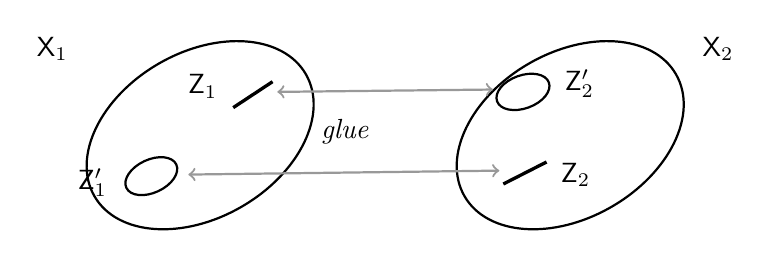
\begin{tikzpicture}[line width=0.8pt]
  \draw[rotate around={30:(0,0)}] (0,0) ellipse (1.55 and 1.05);
  \draw[rotate around={30:(4.7,0)}] (4.7,0) ellipse (1.55 and 1.05);
  \draw[line width=1.2pt] (0.42,0.35) -- (0.92,0.68);
  \node[anchor=east] at (0.35,0.62) {$\mathsf{Z}_1$};
  \draw[rotate around={25:(-0.62,-0.52)}] (-0.62,-0.52) ellipse (0.35 and 0.21);
  \node[anchor=east] at (-1.05,-0.6) {$\mathsf{Z}'_1$};
  \draw[rotate around={20:(4.1,0.55)}] (4.1,0.55) ellipse (0.35 and 0.21);
  \node[anchor=west] at (4.5,0.66) {$\mathsf{Z}'_2$};
  \draw[line width=1.2pt] (3.85,-0.62) -- (4.4,-0.34);
  \node[anchor=west] at (4.45,-0.5) {$\mathsf{Z}_2$};
  \node[anchor=east] at (-1.55,1.1) {$\mathsf{X}_1$};
  \node[anchor=west] at (6.25,1.1) {$\mathsf{X}_2$};
  \draw[gray!80,<->] (0.98,0.55) -- (3.72,0.58);
  \draw[gray!80,<->] (3.8,-0.45) -- (-0.15,-0.5);
  \node at (1.85,0.05) {\textit{glue}};
\end{tikzpicture}
\caption{搭建一个\trProper{}的非射影\trVariety。（依原书手绘图重绘。）}\label{fig:proper-nonprojective-variety}
\end{figure}

那么 $X$ 不是射影的。因为若它是，则它将经由某个\trInvertibleSheaf{} $\mathscr{L}$ 嵌入\trProjectiveSpace。若 $X$ 被嵌入，则 $X_1$ 也被嵌入，于是 $\mathscr{L}$ 限制到 $X_1$ 上必是形如 $\OO_{X_1}(n_1)$ 的\trInvertibleSheaf，其中 $n_1>0$。你可以验证：$\mathscr{L}$ 限制到 $Z_1$ 上是 $\OO_{Z_1}(n_1)$，而 $\mathscr{L}$ 限制到 $Z'_1$ 上是 $\OO_{Z'_1}(2n_1)$。对称地，$\mathscr{L}$ 限制到 $Z_2$ 上是 $\OO_{Z_2}(n_2)$，对某个 $n_2>0$，而 $\mathscr{L}$ 限制到 $Z'_2$ 上是 $\OO_{Z'_2}(2n_2)$。但粘合之后，$Z_1=Z'_2$，且 $Z'_1=Z_2$，于是我们有 $n_1=2n_2$ 与 $2n_1=n_2$，这是不可能的。

\textbf{15.2.12.}\ \emph{沿\trIsomorphic{}的\trClosedSubscheme{}粘合两个\trScheme。}

直截了当地证明：你可以沿\trIsomorphic{}的\trOpenSubscheme{}粘合两个\trScheme。（更精确地说，若 $X_1$ 与 $X_2$ 是\trScheme，分别带有\trOpenSubscheme{} $U_1$ 与 $U_2$，以及一个\trIsomorphism{} $U_1\overset{\sim}{\hookrightarrow}U_2$，那么你可以对「沿 $U_1\overset{\sim}{\hookrightarrow}U_2$ 粘合 $X_1$ 与 $X_2$」讲得通。你应当把这件事想清楚。）类似地，你也可以沿\trIsomorphic{}的\emph{闭}子概形粘合两个\trScheme。我们现在把这件事说精确。设 $Z_1\hookrightarrow X_1$ 与 $Z_2\hookrightarrow X_2$ 是\trClosedEmbedding，而
\[
\phi\colon Z_1\overset{\sim}{\longrightarrow}Z_2
\]
是一个\trIsomorphism。我们将解释如何沿 $\phi$ 把 $X_1$ 粘合到 $X_2$ 上。其结果将被称为 $X_1\amalg_\phi X_2$。

\textbf{15.2.13.}\ \emph{动机示例。}\quad 我们的动机示例是：若 $X_i=\Spec A_i$，$Z_i=\Spec A_i/I_i$，而 $\phi$ 对应于 $\phi^{\sharp}\colon A_2/I_2\overset{\sim}{\longrightarrow}A_1/I_1$。那么其结果将是 $\Spec R$，其中 $R$ 是由那些「经由 $\phi$ 相合」的有序对 $(a_1,a_2)\in A_1\times A_2$ 组成的\trRing。更精确地说，这是一个环的\trFiberProduct：
\[
R:=A_1\times_{\phi^{\sharp}\colon A_1/I_1\to A_2/I_2}A_2.
\]

\textbf{15.2.14.}\ \emph{一般构造，作为一个\trLocallyRingedSpace。}\quad 在我们的一般情势下，我们或许希望用这种形式的开片盖住 $X_1$ 与 $X_2$。那样我们将不得不为粘合与选取而操心，所以为了避免这些，我们改为先把 $X_1\amalg_\phi X_2$ 作为一个\trLocallyRingedSpace{}构造出来。作为一个\trTopologicalSpace，其定义是清楚的：把二者的\trUnderlyingSet{}沿着 $Z_1\cong Z_2$ 的\trUnderlyingSet{}粘合起来，并给这个粘合而成的集合赋予\trTopology，使得 $X_1\amalg_\phi X_2$ 的一个子集是\trOpen{}的，当且仅当它限制到 $X_1$ 与 $X_2$ 上都是\trOpen{}的。为方便起见，令 $Z$ 为 $Z_1$（或者，等价地，$Z_2$）在 $X_1\amalg_\phi X_2$ 中的\trImage。接下来，我们在每个点 $p\in X_1\amalg_\phi X_2$ 处定义\trStructureSheaf{}的\trStalk。若 $p\in X_i\setminus Z=(X_1\amalg_\phi X_2)\setminus X_{3-i}$（希望这一点含义是清楚的），我们便把\trStalk{}定义为 $\OO_{X_i,p}$。若 $p\in X_1\cap X_2$，我们把\trStalk{}定义为由那些在 $\OO_{Z_1,p}\cong\OO_{Z_2,p}$ 中相合的元素 $(s_1,s_2)\in\OO_{X_1,p}\times\OO_{X_2,p}$ 组成。如果你能完成下面这道练习，本段中一切的含义对你来说都会是清楚的。

\textbf{15.2.J.（练习）}\quad 用\trCompatibleGerm{}定义 $\OO_{X_1\amalg_\phi X_2}$ 的\trStructureSheaf。（芽\trCompatible{}应当是什么意思？提示：对 $z\in Z$，设我们有 $X_1$ 的\trOpenSubset{} $U_1$ 与 $X_2$ 的\trOpenSubset{} $U_2$，满足 $U_1\cap Z=U_2\cap Z$，于是 $U_1$ 与 $U_2$ 粘合起来给出 $X_1\amalg_\phi X_2$ 的一个\trOpenSubset{} $U$。又设我们在 $U_1$ 上有函数 $f_1$、在 $U_2$ 上有函数 $f_2$，它们「在 $U\cap Z$ 上相合」——这是什么意思？那么我们就宣称：「把 $f_1$ 与 $f_2$ 粘合起来而在 $U$ 上得到的函数」的诸\trGerm{}是\trCompatible{}的。）证明：所得到的\trRingedSpace{}是一个\trLocallyRingedSpace。

接下来我们想证明：\trLocallyRingedSpace{} $X_1\amalg_\phi X_2$ 是一个\trScheme。显然它在远离 $Z$ 处是一个\trScheme。我们先验证一个特例。

\textbf{15.2.K.（练习）}\quad 证明：在\mbox{例~15.2.13} 中，\S15.2.14 的构造确实给出 $\Spec(A_1\times_{\phi^{\sharp}}A_2)$。

\textbf{15.2.L.（练习）}\quad 在一般情形，设 $x\in Z$。证明：存在一个\trAffine\trOpenSubset{} $\Spec A_1\subset X_1$，使得 $Z\cap\Spec A_1=Z\cap\Spec A_2$。然后用\mbox{练习~15.2.J} 证明：$X_1\amalg_\phi X_2$ 在 $x$ 的一个\trOpen\trNeighborhood{}中是一个\trScheme，从而是一个\trScheme。

\textbf{15.2.15.}\ \emph{\trhRemark{}。}

（a）正如记号所暗示的，这是\trScheme{}的\trCategory{}中的一个\trFiberedCoproduct，而且实际上在\trLocallyRingedSpace{}的\trCategory{}中也是如此。我们并不需要这个事实，但你若愿意可以证明它；这并不难。与积的情状不同，\trFiberedCoproduct{}在\trScheme{}的\trCategory{}中一般并不存在。神奇的是（并且出于对\trScheme{}而言特殊的原因），所得的余纤维图表同时也是一个\emph{纤维}（fibered，即\trCartesianDiagram）图表。这有令人愉快的推论。例如，这个构造「对平坦\trBaseChange{}表现良好」（或者说与平坦\trBaseChange{}「交换」）。

（b）你或许会希望：若你有一个\trScheme{} $X$，带着两个不相交的\trClosedSubscheme{} $W'$ 与 $W''$，以及一个\trIsomorphism{} $W'\overset{\sim}{\longrightarrow}W''$，那么你应当能够沿 $W'\to W''$ 把 $X$ 与自身粘合起来。这个构造行不通，而且的确可能根本办不到。你仍然可以把这个商作为一个\trAlgebraicSpace{}来讲得通，我们不打算在这里定义它。

\textbf{15.2.M.（练习）}\quad 我们继续使用记号 $X_i$、$\phi$ 等等。设我们在 $A$-\trScheme{}的\trCategory{}中工作。

（a）若 $X_1$ 与 $X_2$ 都是\trUniversallyClosed{}的，证明 $X_1\amalg_\phi X_2$ 亦然。

（b）若 $X_1$ 与 $X_2$ 都是\trSeparated{}的，证明 $X_1\amalg_\phi X_2$ 亦然。

（c）若 $X_1$ 与 $X_2$ 都是在\trNoether\trRing{} $A$ 上\trFiniteType{}的，证明 $X_1\amalg_\phi X_2$ 亦然。（提示：化归到\mbox{动机示例~15.2.13} 的「\trAffine」情形。选取 $A_1$ 的\trGenerator{} $x_1,\dots,x_n$ 与 $y_1,\dots,y_n$，使得经由 $\phi$，$x_i$ 模 $I_1$ 与 $y_i$ 模 $I_2$ 相合。选取 $I_2$ 的\trGenerator{} $g_1,\dots,g_m$——这里要用到 $A$ 的诺特性。证明 $(x_i,y_i)$ 与 $(0,g_i)$ 生成 $R\subset A_1\times A_2$，如下。设 $(a_1,a_2)\in R$\footnote{原书此处作「$(a,b)\in(A,B)$」，其中 $(A,B)$ 当系 $A\times B$ 之误（该二元组系 $R\subset A_1\times A_2$ 中元素），径改。——译者注}。那么存在某个多项式 $m$ 使得 $a_1=m(x_1,\dots,x_n)$。于是对某个 $a'_2\in I_2$，$(a_1,a_2)-m((x_1,y_1),\dots,(x_n,y_n))=(0,a'_2)$。而这个 $a'_2$ 可以写成 $\sum_{i=1}^m\ell_i(y_1,\dots,y_n)g_i$。但随后 $(0,a'_2)=\sum_{i=1}^m\ell_i((x_1,y_1),\dots,(x_n,y_n))(0,g_i)$。）

于是若 $X_1$ 与 $X_2$ 都是\trProper{}的，则 $X_1\amalg_\phi X_2$ 亦然。

另一方面，我们刚刚看到（\S15.2.11）：若 $X_1$ 与 $X_2$ 都是\emph{射影}的，则 $X_1\amalg_\phi X_2$ 未必射影。

\textbf{15.2.16.}\ \emph{玩转更一般的概形「粘合」（\trCoproduct）。}\quad 若你读到了这里，你就可以相当廉价地看到更多有意思的例子。设更一般地，你有一个\trClosedEmbedding{} $Z\hookrightarrow Y$，而只有一个\trAffine\trMorphism{} $Z\to X$。我们仍然可以沿 $Z$ 把 $X$ 与 $Y$「粘合」起来得到一个\trScheme{} $W$，做法是遵循同一个配方。

\textbf{15.2.N.（扩展练习）}\quad 给定一个\trClosedEmbedding{} $\alpha\colon Z\hookrightarrow X$ 与一个\trAffine\trMorphism{} $\beta\colon Z\to Y$，证明（遵循 \S15.2.12 的策略）：存在一张概形的\trFiberedCoproduct{}方图
\begin{equation*}\tag{15.2.16.1}\label{eq:pushout-square-schemes}
\begin{tikzcd}[column sep=3.5em, row sep=3.5em]
Z \ar[r, "\beta\;\text{仿射}"] \ar[d, hook, "\alpha\;\text{闭嵌入}"] & Y \ar[d, "\alpha'"'] \\
X \ar[r, "\beta'"] & W.
\end{tikzcd}
\end{equation*}
这张方图在相差唯一\trIsomorphism{}的意义下必然唯一。

\textbf{15.2.O.（练习）}\quad 证明：\eqref{eq:pushout-square-schemes} 同时也是一个拉回方图（即\trCartesianDiagram），并且 $\alpha'$ 是一个\trClosedEmbedding，$\beta'$ 是一个\trAffine\trMorphism。

\textbf{15.2.17.}\ \emph{一个没有\trClosedPoint{}的\trScheme。}

在求解\mbox{扩展练习~15.2.N} 的过程中，你将会研究那个（容易得多的）\trAffine{}情形，它对应于下面这张环的方图。
\begin{equation*}\tag{15.2.17.1}\label{eq:pushout-square-rings}
\begin{tikzcd}[column sep=4.5em, row sep=3.5em]
A/I & B \ar[l, "\beta^{\sharp}"] \\
A \ar[u] & A\times_{A/I}B \ar[l] \ar[u]
\end{tikzcd}
\end{equation*}

于是对应于 $W$ 的那个环可以被解读为
\[
A\times_{A/I}B=\{(a,b)\in A\times B : a\equiv\alpha^{\sharp}(b)\pmod{I}\}.
\]

我们可以用这个构造来看到一些有意思的行为。例如，我们现在来描述一个没有\trClosedPoint{}的\trScheme{} $X$。它将有可数多个点 $\{p_1,p_2,\dots\}$，而它的诸\trOpenSet{}将形如 $\{p_1,\dots,p_n\}$。（显然这个\trTopologicalSpace{}没有\trClosedPoint{}。）每个\trOpenSet{}都将是\trAffine{}的：$\{p_1,\dots,p_n\}=\Spec A_n$。我们如下归纳地构造 $A_n$。令 $A_1=k(x_1,x_2,\dots)$（\trField{} $k$ 的一个可数生成超越扩张）。我们归纳地构造 $A_{n+1}$，用的是 \eqref{eq:pushout-square-rings} 的如下特例：
\[
\begin{tikzcd}[column sep=7.5em, row sep=3.5em]
k(x_n,x_{n+1},\dots) & k(x_{n+1},x_{n+2},\dots)[x_n]_{x_n} \ar[l, hook] \\
A_n \ar[u] & A_{n+1} \ar[l, hook] \ar[u]
\end{tikzcd}
\]
顶上一行不过是一个\trDVR{}映入其\trFractionField{} $K$。左面一列是一个复杂的\trLocalRing，其\trResidueField{}正是同一个域 $K$。

把注意力集中在 $\{p_1,p_2,p_3\}$ 上时，这件事可能更容易理解。令 $F=k(x_3,x_4,\dots)$。那么 $A_1$ 是一个\trField，$A_2$ 是\trDVR{} $F(x_2)[x_1]_{x_1}$，而 $A_3$ 是 $A_2$ 的一个\trSubring，其模 $x_1$ 的剩余落在\trDVR{} $F[x_2]_{x_2}$ 之中。（环 $A_3$ 是一个\emph{\trRank{} $2$ \trValuationRing}的例子；你能看出它为何配得上这个名字吗？）

\textbf{15.2.P.（练习）}\quad 利用上述内容描述一个没有\trClosedPoint{}的\trScheme{} $\bigcup_{n\ge 1}\Spec A_n$。



\section{曲线到射影的延拓定理}

现在，我们要用上一节的主定理——\mbox{定理~15.2.2}——来证明一个有用而具体的结果。（事实上，我们本可以早得多就证明它——只要稍加巧思，你就可以把对\mbox{定理~15.2.2} 的援引换成\mbox{练习~7.3.M}，并且一旦认识了\trDVR，便能证明它。）

作为动机，我们来考虑 \S15.2 开头那个例子的一个变体：\eqref{eq:cubic-map-failed} 是一次想要得到\trMorphism{} $\mathbb{P}^2_k\to\mathbb{P}^3_k$ 的失败尝试。这个例子用 $\mathbb{P}^2_k$ 而非 $\mathbb{P}^1_k$ 作为源，是有一番道理的。举例来说，乍看之下，由
\[
[x^7,\; x^3y^4,\; x^4y^3+4x^5y^2,\; x^5y^2+x^7]
\]
给出的\trRationalMap{} $\mathbb{P}^1_k\dashrightarrow\mathbb{P}^3_k$ 似乎并不给出一个\trMorphism{} $\mathbb{P}^1_k\to\mathbb{P}^3_k$，因为它在 $[x,y]=[0,1]$ 处没有定义。但我们其实可以把这个映射延拓到 $[0,1]$ 之上，用的是
\begin{equation*}\tag{15.3.0.1}\label{eq:curve-proj-divided}
[x^7,\; x^3y^4,\; x^4y^3+4x^5y^2,\; x^5y^2+x^7]=[x^4,\; y^4,\; xy^3+4x^2y^2,\; x^2y^2+x^4]
\end{equation*}
——我们只消通除以 $x^3$，便能叫这个\trMorphism{}讲得通。类似地，$[x^2,x^{-2}y^4,x^{-1}y^3+4y^2,y^2+x^2]$ 看上去同样在 $[x,y]=[0,1]$ 处没有定义，但你可以看出该怎么办（以及它为何能延拓成与 \eqref{eq:curve-proj-divided} 相同的映射）。这将推广成下面的结果。

\textbf{15.3.1.\ 曲线到射影的延拓定理。}\ ——\ \emph{设 $C$ 是仿射\trBaseScheme{} $S=\Spec A$ 上\trPureDimension{} $1$ 的一个\trNoetherian{}概形，而 $p\in C$ 是它的一个正则\trClosedPoint。设 $Y$ 是一个射影 $S$-\trScheme。那么，任何\trMorphism{} $C\setminus\{p\}\to Y$（$S$-\trScheme{}之间的\trMorphism）都可延拓到整个 $C$ 上。}

为预先杜绝任何混淆：这里的 $C$ 是「绝对\trPureDimension{} $1$」，而非相对\trPureDimension{} $1$。

实际使用中，我们将在 $S=\Spec k$、而 $C$ 是一个 $k$-\trVariety{}时使用这条定理。我们假定 $S$ 仿射的唯一理由是：在知道什么是射影\trMorphism{}之前（\S17.3），我们还不会知道「射影 $S$-\trScheme」的含义。而一旦知道了这条陈述的含义，下面的证明便立即推广到一般的 $S$。

注意：这样的延拓若存在，必是唯一的：$C$ 的非既约\trLocus{}是一个\trClosedSubset（练习~6.6.N）。于是，把 $C$ 换成 $p$ 的一个既约的\trOpen\trNeighborhood{}之后，我们便可以运用「既约到分离」定理~11.3.2，即：从既约概形到分离概形的\trMorphism{}由其在某个\trDense\trOpenSubset{}上的行为所确定。另一种说法是：映入分离概形的\trMorphism{}越过某个\trEffectiveCartierDivisor{}的延拓至多只有一种方式（\mbox{练习~11.3.G}）。

下面的练习表明，这些假设都是必要的。

\textbf{15.3.A.（练习）}\quad 在以下每一种情形中，证明：\trMorphism{} $C\setminus\{p\}\to Y$ 都无法延拓为\trMorphism{} $C\to Y$。

（a）\emph{$Y$ 的射影性是必要的。}设 $C=\mathbb{A}^1_k$，$p=0$，$Y=\mathbb{A}^1_k$，而 $C\setminus\{p\}\to Y$ 由「$t\mapsto 1/t$」给出。

（b）\emph{$C$ 的一维性是必要的。}设 $C=\mathbb{A}^2_k$，$p=(0,0)$，$Y=\mathbb{P}^1_k$，而 $C\setminus\{p\}\to Y$ 由 $(x,y)\mapsto[x,y]$ 给出。

（c）\emph{$C$ 的非奇异性是必要的。}设 $C=\Spec k[x,y]/(y^2-x^3)$，$p=0$，$Y=\mathbb{P}^1_k$，而 $C\setminus\{p\}\to Y$ 由 $(x,y)\mapsto[x,y]$ 给出。

我们指出：把这条（容易的）定理与（艰难的）\trProperness{}的\trValuativeCriteria（\mbox{定理~13.7.6}）结合起来，便可以绕开（棘手但并不艰难的）\mbox{\trFundamentalTheoremOfEliminationTheory~8.4.10}，得到\trProjectiveSpace{}之\trProperness{}的一个证明（见\mbox{练习~13.7.F}）。更花哨的注记：\trProperness{}的\trValuativeCriteria{}还可以用来证明：若只要求 $Y$ 是\trProper{}的，\mbox{定理~15.3.1} 依然为真，但这需要花些心思。

\textbf{15.3.2.}\ \emph{证明的中心想法。}\quad 这个证明的中心想法可以概括为「去分母」，而下面的动机示例正说明了它。假设你有一个从 $\mathbb{A}^1\setminus\{0\}$ 到\trProjectiveSpace{}的\trMorphism，而你想把它延拓到 $\mathbb{A}^1$ 上。假设这个映射由 $t\mapsto[t^4+t^{-3},t^{-2}+4t]$ 给出。那么你当然会「去分母」，把映射换成 $t\mapsto[t^7+1,t+4t^4]$。类似地，若映射由 $t\mapsto[t^2+t^3,t^2+t^4]$ 给出，你就会除以 $t^2$，得到映射 $t\mapsto[1+t,1+t^2]$。

\textbf{15.3.3.}\ \emph{证明。}\quad 我们的计划是设法把自己挪进这样一种境地：能够应用 \S15.3.2 的想法。我们先做几个快速的化归。$C$ 的非既约\trLocus{}是闭的（\mbox{练习~6.6.N}）且不含 $p$，于是把 $C$ 换成 $p$ 的一个适当的\trOpen\trNeighborhood{}之后，便可不妨设 $C$ 既约且仿射。

接下来，我们化归到 $Y=\mathbb{P}^n_A$ 的情形。选取一个\trClosedEmbedding{} $Y\to\mathbb{P}^n_A$。若该结果对 $\mathbb{P}^n$ 成立，而我们有一个\trMorphism{} $C\to\mathbb{P}^n$ 使 $C\setminus\{p\}$ 映入 $Y$，则 $C$ 也必映入 $Y$。理由：我们可以化归到源是某个\trAffine\trOpenSubset、目标是 $\mathbb{A}^n_A\subset\mathbb{P}^n_A$（从而仿射）的情形。这时，在 $Y\cap\mathbb{A}^n_A$ 上消失的那些函数拉回到 $C$ 上，便成为在 $C$ 的诸\trIrreducibleComponent{}的诸\trGenericPoint{}处消失的函数，从而在 $C$ 上处处消失（利用 $C$ 的既约性）；也就是说，$C$ 映入 $Y$。

选取 $C$ 在 $p$ 处的\trLocalRing{}中的一个\trUniformizer{} $t\in\mathfrak{m}\setminus\mathfrak{m}^2$。由于 $t$ 是 $p$ 的某个\trNeighborhood{}上的函数，把 $C$ 换成这个\trNeighborhood{}之后，便可不妨设 $t$ 是 $C$ 上的一个函数。于是 $V(t)$ 包含 $p$（因为 $t\in\mathfrak{m}$），但 $V(t)$ 不包含 $C$ 中含 $p$ 的那条\trIrreducibleComponent（因为 $t\notin\mathfrak{m}^2$）；因此，把 $C$ 换成它在 $(C\setminus V(t))\cup\{p\}$ 中 $p$ 的一个仿射\trOpen\trNeighborhood——注意 $(C\setminus V(t))\cup\{p\}\subset C$ 是开集，因为 $C$（几乎）具有\trCofiniteTopology\footnote{译注：这正是「几乎」的含义——$C$ 的真闭子集若不含整条\trIrreducibleComponent，便只是有限个点。}——我们便可不妨设 $p$ 是函数 $t$ 唯一的\trZeros（并且，当然，$t$ 在 $p$ 处以\trMultiplicity{} $1$ 消失）。

我们有一个映射 $C\setminus\{p\}\to\mathbb{P}^n_A$，由\mbox{定理~15.2.2}，它对应于 $C\setminus\{p\}$ 上的一个\trLineBundle{} $\mathscr{L}$ 以及它的 $n+1$ 个在 $C\setminus\{p\}$ 中无公共\trZeros{}的\trSection。取 $C\setminus\{p\}$ 的一个非空\trOpen{}集 $U$，使 $\mathscr{L}\cong\OO$。于是，把 $C$ 换成 $U\cup\{p\}$ 之后，我们可以把到 $\mathbb{P}^n$ 的这个映射解读为 $n+1$ 个\emph{\trRationalFunction} $f_0,\dots,f_n$，它们在除去 $p$ 之处有定义\footnote{原书此处作（defined away away from $p$），「away」重出，当为衍文，径删。——译者注}，并且在除去 $p$ 之处没有公共\trZeros。令 $N=\min_i(\mathrm{val}_p f_i)$。则 $t^{-N}f_0,\dots,t^{-N}f_n$ 是 $n+1$ 个没有公共\trZeros{}的函数。于是它们确定一个\trMorphism{} $C\to\mathbb{P}^n_A$，如愿地延拓了 $C\setminus\{p\}\to\mathbb{P}^n_A$。\hfill$\square$

\textbf{15.3.B.（练习；有用的锻炼）}\quad 设 $X$ 是一个\trNoetherian{} $k$-\trScheme，而 $Z$ 是一个\trIrreducible{}的余维数 $1$ 的\trSubvariety，其\trGenericPoint{}是 $X$ 的一个\trRegular{}点（于是\trLocalRing{} $\OO_{X,Z}$ 是一个\trDVR）。设 $\pi\colon X\dashrightarrow Y$ 是到某个射影 $k$-\trScheme{}的一个\trRationalMap。证明：该\trRationalMap{}的\trDomainOfDefinition{}包含 $Z$ 的一个\trDense\trOpenSubset。换言之，从\trNoetherian{} $k$-\trScheme{}到射影 $k$-\trScheme{}的\trRationalMap{}可以在正则的余维数 $1$ 的集合上延拓。（我们此前已经见过这条原理在起作用——见关于\trCremona{}变换的\mbox{练习~7.5.J}。）

\textbf{15.3.4.}\ \hard\ \textbf{扩展示例：正则平面\trCurve{}的\trTangentLine{}是\trSecant（secant）的极限。}

我们现在来讨论一个扩展示例，它或许能对许多不同的事情给出洞察。在学习微积分时，我们有时被教导：平面\trCurve{}的\trTangentLine{}是\trSecant{}的极限。如今我们可以在\mbox{曲线到射影的延拓定理~15.3.1}\footnote{原书此处作（The Curve-to-Projective Extension Theorem 11.1.1），编号 11.1.1 当系 15.3.1 之误（该定理即本节定理 15.3.1），径改。——译者注} 的框架下看待这件事，$\delta$ 与 $\varepsilon$ 由此变成了容易的代数。这段讨论还预示了\trDiagonalMorphism{}在理解\trDifferential{}时的重要性。

设 $k$ 是一个\trField，你起初不妨把它取为\trAlgClosed{}的。（日后你可以思考：这一切在任意\trField{}上如何讲得通。）设 $C\subset\mathbb{A}^2_k$ 是一条平面\trCurve，由方程 $f(x,y)=0$ 给出。取定 $C$ 的一个点 $p=(x_0,y_0)$。给定 $C$ 的一个点 $q=(x_1,y_1)$，设 $x_1\ne x_0$，则联结二者的直线的斜率是 $m=(y_1-y_0)/(x_1-x_0)$，而联结二者的直线的方程是
\[
(y-y_0)=\frac{y_1-y_0}{x_1-x_0}(x-x_0).
\]

更一般地（即便 $x_1=x_0$ 也可，但仍要求 $y_1\ne y_0$），联结二者的直线具有「斜率」$[x_1-x_0,y_1-y_0]\in\mathbb{P}^1_k$，而联结二者的直线的方程是 $(x_1-x_0)(y-y_0)=(y_1-y_0)(x-x_0)$。于是我们有一个映射
\begin{equation*}\tag{15.3.4.1}\label{eq:secant-slope-map}
C\setminus p\longrightarrow\mathbb{P}^1_k
\end{equation*}
它把 $q$ 送到\trSecant $\overline{pq}$ 的「斜率」。\mbox{曲线到射影的延拓定理~15.3.1} 说：只要 $p$ 是 $C$ 的一个\trSmooth{}点，这个映射便可越过 $p$ 延拓。我们来把代数算出来。请记住，此时 $x_0,y_0\in k$，因为 $p$ 是取定的点。定义 $F(x_1,y_1):=f(x_1,y_1)-f(x_0,y_0)\in k[x_1,y_1]$。

\textbf{15.3.C.（练习）}\quad 证明：$F\in(x_1-x_0,y_1-y_0)$。

于是我们可以把 $F$ 写成 $g(x_1,y_1)(x_1-x_0)+h(x_1,y_1)(y_1-y_0)$，其中 $g,h\in k[x_1,y_1]$ 的某种选取（不必唯一）。请取定这样一个 $g$ 与 $h$。

\textbf{15.3.D.（练习）}\quad 证明：若 $p=(x_0,y_0)$ 是 $C$ 的\trSmooth{}点，且带有非竖直的\trTangentVector，则 $h(x_0,y_0)\ne 0$。

\textbf{15.3.E.（练习）}\quad 证明：若 $p=(x_0,y_0)$ 是 $C$ 的\trSmooth{}点，则 $p$ 处\trTangentLine{}的斜率是 $[-h(x_0,y_0),g(x_0,y_0)]\in\mathbb{P}^1_k$，而\trTangentLine{}的方程是
\[
g(x_0,y_0)(x-x_0)+h(x_0,y_0)(y-y_0)=0.
\]



\section{难而重要：线丛与\trWeilDivisor}

\trWeilDivisor{}这一概念，为理解与分类\trLineBundle{}提供了一条极好的途径。在动工之前，应当先警告你：这是\trAlgebraicGeometry{}中那种难以消化的话题之一——学会它，会改变你思考\trLineBundle{}的方式。可是一旦你用顺了手这本通往除子的不完善词典，它便成了你的第二天性。

在本节中，我们只考虑\emph{\trNoetherian{}正规\trScheme}。这样做是因为：我们将要用到\trIrreducibleComponent{}的有限分解（\mbox{练习~5.3.B}）、\trDVR{}的性质（\S13.5），以及代数\trHartogs{}引理~13.5.19。我们所讨论的内容有些在更一般的情形下也成立；我们诚邀专家通过对各条陈述审慎地减弱假设，来考虑种种推广。

\textbf{15.4.1.}\ \emph{\trhDefinition{}。}\quad 把 $X$ 上的一个\textbf{\trWeilDivisor}（Weil divisor）定义为 $X$ 的余维数 $1$ 不可约\trClosedSubset{}的形式 $\mathbb{Z}$-线性组合。换言之，$X$ 上的一个\trWeilDivisor{}被定义为如下形式的对象
\[
\sum_{Y\subset X\text{ 余维数 }1}n_Y[Y],
\]
其中诸 $n_Y$ 是整数，且除有限多个之外全为零。\trWeilDivisor{}显然构成一个\trAbelian\trGroup，记作 $\operatorname{Weil}\,X$。例如，若 $X$ 是一条\trCurve，则\trWeilDivisor{}就是闭点的线性组合。

\textbf{15.4.2.}\quad 我们称 $[Y]$ 为一个\textbf{不可约除子}（irreducible (Weil) divisor）。若\trWeilDivisor{} $\mathrm{D}=\sum n_Y[Y]$ 满足对一切 $Y$ 都有 $n_Y\ge 0$，则称它是\textbf{有效的}（effective）。此时我们写 $\mathrm{D}\ge 0$，而 $\mathrm{D}_1\ge\mathrm{D}_2$ 意指 $\mathrm{D}_1-\mathrm{D}_2\ge 0$。\trWeilDivisor{} $\mathrm{D}$ 的\textbf{\trSupport}记作 $\operatorname{Supp}\,\mathrm{D}$，它是子集 $\cup_{n_Y\ne 0}Y$。若 $U\subset X$ 是一个\trOpenSet，我们定义\textbf{\trRestrictionMap} $\operatorname{Weil}\,X\to\operatorname{Weil}\,U$ 为 $\sum n_Y[Y]\mapsto\sum_{Y\cap U\ne\varnothing}n_Y[Y\cap U]$。

\textbf{15.4.A.（容易的练习）}\quad 证明：$\mathbb{P}^n_k$ 上的不可约除子，恰与 $k[x_0,\dots,x_n]$ 中的不可约\trHomogeneous{}多项式相对应（在相差非零纯量 $k^{\times}$ 倍乘的意义下）。

\textbf{15.4.3.}\quad 设 $\mathscr{L}$ 是一个\trInvertibleSheaf，而 $s$ 是 $\mathscr{L}$ 的一个\trRational\trSection，它不在 $X$ 的任何\trIrreducibleComponent{}上处处为零。（\trRational\trSection{}由 $X$ 的一个\trDense\trOpenSubset{}上的\trSection{}给出，并配有显而易见的等价关系，见 \S14.2.1。）

我们不妨按下述方式理解 $s$ 沿一个不可约\trWeilDivisor{} $Y$ 的\textbf{\trValuation}——记作 $\operatorname{val}_Y(s)$。取任意一个包含 $Y$ 的\trGenericPoint{}、且其上 $\mathscr{L}$ 可平凡化的\trOpenSet{} $U$，连同 $U$ 上任取的一个\trTrivialization；在这个\trTrivialization{}之下，$s$ 成为 $U$ 上的一个非零\trRationalFunction，从而拥有一个\trValuation（\S13.5.14）。任何两个这样的\trTrivialization{}都相差一个可逆函数（\trTransitionFunction{}必是可逆的），故此\trValuation{}是\trWellDefined{}的。注意，由\mbox{练习~13.5.G}，对除有限多个之外的一切 $Y$，都有 $\operatorname{val}_Y(s)=0$。

于是 $s$ 确定了一个\trWeilDivisor
\[
\operatorname{div}(s):=\sum_Y\operatorname{val}_Y(s)[Y].
\]
求和跑遍 $X$ 的全部不可约除子 $Y$。我们称 $\operatorname{div}(s)$ 为\trRational\trSection{} $s$ 的\textbf{零点与极点除子}（divisor of zeros and poles）（参看\mbox{定义~13.5.7}）。

\textbf{15.4.4.\ 「带\trRational\trSection{}的\trLineBundle」这一重要群。}\quad 现在考虑集合 $\{(\mathscr{L},s)\}$，其元素是「\trLineBundle{} $\mathscr{L}$ 连同 $\mathscr{L}$ 的一个\trRational\trSection{} $s$，且 $s$ 在 $X$ 的任何\trIrreducibleComponent{}上都不是零\trSection」这样的对子，并在\emph{同构}的意义下视作相同。（同构 $(\mathscr{L},s)\cong(\mathscr{L}',s')$ 意指线丛的一个同构，它把 $s$ 送到 $s'$。）这个集合（对同构取商之后）在张量积 $\otimes$ 之下构成一个\trAbelian\trGroup，其单位元是 $(\OO_X,1)$。（刁钻的小问题：$(\mathscr{L},s)$ 在这个群中的逆是什么？）

应当注意到：若 $t$ 是 $X$ 上的一个可逆函数，则用 $t$ 相乘便给出一个同构
\[
(\mathscr{L},s)\overset{\sim}{\longleftrightarrow}(\mathscr{L},st).
\]
类似地，$(\mathscr{L},s)/(\mathscr{L},u)=(\OO,s/u)$。此处 $s/u$ 是一个有理\emph{函数}。

映射 $\operatorname{div}$ 给出一个群同态
\begin{equation*}\tag{15.4.4.1}\label{eq:div-group-homomorphism}
\operatorname{div}\colon\{(\mathscr{L},s)\}/\text{同构}\longrightarrow\operatorname{Weil}\,X.
\end{equation*}

\textbf{15.4.B.（更容易的练习）}\quad
（a）\emph{（有理函数的除子）}\quad 验证：在 $\mathbb{A}^1_k$ 上，$\operatorname{div}\bigl(x^3/(x+1)\bigr)=3[(x)]-[(x+1)]$（「$=3[0]-[-1]$」）。
（b）\emph{（一个非平凡\trInvertibleSheaf{}的\trRational\trSection{}的除子）}\quad 在 $\mathbb{P}^1_k$ 上，存在一个「对应于」$x^2/(x+y)$ 的 $\OO(1)$ 的\trRational\trSection。弄清楚这是什么意思，并算出 $\operatorname{div}\bigl(x^2/(x+y)\bigr)$。

\eqref{eq:div-group-homomorphism} 这个同态，将是确定许多 $X$ 上全部\trLineBundle{}的关键。（注意：任何\trInvertibleSheaf{}都会有这样一个\trRational\trSection。对每个\trIrreducibleComponent{}，取一个不与任何其他\trIrreducibleComponent{}相遇的非空\trOpenSet；再把它缩小，使 $\mathscr{L}$ 成为平凡；选定一个\trTrivialization；然后取所有这些\trOpenSet{}的并，并在其上选定在\trTrivialization{}之下对应于 $1$ 的那个\trSection。）我们将会看到，在合理的情势下，这个映射 $\operatorname{div}$ 将是\trInjectiveMap{}的，并且常常是一个\trIsomorphism。于是，通过忘掉\trRational\trSection（亦即，取一个适当的商），我们便将刻画出全部\trLineBundle{}的\trPicardGroup。让我们把这一策略付诸行动。

\textbf{15.4.5.\ \trhProposition{}。}\ ——\ \emph{若 $X$ 正规且\trNoetherian，则映射 $\operatorname{div}$ 是单射。}

\emph{证明。}\quad 设 $\operatorname{div}(\mathscr{L},s)=0$。那么 $s$ 没有\trPole。由\mbox{练习~14.2.F}，$s$ 是一个\trRegular\trSection。现在我们来证明：态射 $\times s\colon\OO_X\to\mathscr{L}$ 事实上是一个\trIsomorphism；这便将证得本命题，因为它给出一个同构 $(\OO_X,1)\overset{\sim}{\longleftrightarrow}(\mathscr{L},s)$。

只需证明：在 $X$ 的一个 $\mathscr{L}$ 为平凡的开子集 $U$ 上 $\times s$ 是同构即可，因为 $X$ 被 $\mathscr{L}$ 的平凡化邻域所覆盖（因 $\mathscr{L}$ 局部平凡）。选取一个同构 $i\colon\mathscr{L}\vert_U\overset{\sim}{\longrightarrow}\OO_U$。把 $\times s$ 与 $i$ 复合，便得到映射 $\times s'\colon\OO_U\to\OO_U$，它是乘以某个有理函数 $s'=i(s)$ 的乘法，而这个函数既无\trZeros{}也无\trPole。有理函数 $s'$ 是正则的，因为它没有\trPole（\mbox{练习~13.5.I}），同理 $1/s'$ 也是正则的。于是 $s'$ 是 $U$ 上的一个可逆函数，故 $\times s'$ 是同构。从而 $\times s$ 在 $U$ 上是同构。\hfill$\square$

受此启发，我们试图找出 $\operatorname{div}$ 的一个逆，或至少确定 $\operatorname{div}$ 的像。

\textbf{15.4.6.\ 重要定义：$\OO_X(\mathrm{D})$。}\quad \emph{现在设 $X$ 是正规的}——这将是本节其余部分的一条\trStandingHypothesis。

再设 $X$ 是不可约的（这纯粹是为了免得 \eqref{eq:oxd-sections-definition} 看上去更丑——不过你尽可放松这条假设；见\mbox{练习~15.4.C}）。若有帮助的话：回想正规概形是若干个不可约正规概形的\trDisjointUnion（\mbox{练习~5.4.B}）——所以这条假设着实无害。

设 $\mathrm{D}$ 是一个\trWeilDivisor。定义层 $\OO_X(\mathrm{D})$ 为
\begin{equation*}\tag{15.4.6.1}\label{eq:oxd-sections-definition}
\Gamma(U,\OO_X(\mathrm{D})):=\{t\in K(X)^{\times}\ :\ \operatorname{div}\vert_U t+\mathrm{D}\vert_U\ge 0\}\cup\{0\}.
\end{equation*}
此处 $\mathrm{D}\vert_U$ 是 $\mathrm{D}$ 到 $U$ 上的\trRestriction（定义见 \S15.4.2），而 $\operatorname{div}\vert_U t$ 意指把 $t$ 视为 $U$ 上的\trRationalFunction{}所取的除子（亦即，只考虑 $U$ 的那些不可约除子）。当上下文清楚时，$\OO_X(\mathrm{D})$ 中的下标 $X$ 将被省去。$\OO_X(\mathrm{D})$ 在 $U$ 上的诸\trSection，就是那些「\trPole{}与\trZeros{}被 $\mathrm{D}$ 约束」的 $U$ 上的\trRationalFunction：$\mathrm{D}$ 中的一个正系数允许一个该阶的\trPole；一个负系数则要求一个该阶的\trZeros。在 $\mathrm{D}$ 的\trSupport{}之外，它（同构地）就是\trStructureSheaf（由代数\trHartogs{}引理~13.5.19）。

\textbf{15.4.7.}\ \emph{重要注记。}\quad 注意到下面这件事将是至关重要的：$\OO_X(\mathrm{D})$ 自带一个对应于 $1\in K(X)^{\times}$ 的、典范的非零「有理截面」。（说它是有理截面，是因为它是某个稠密开集——也就是 $\operatorname{Supp}\,\mathrm{D}$ 的补集——上的截面。）

\textbf{15.4.C.（较不重要的练习）}\quad 把 $\OO_X(\mathrm{D})$ 的定义推广到 $X$ 未必不可约的情形。（这只是一个语言问题。做完之后，你尽可在本节其余部分抛弃这条假设。）

\textbf{15.4.D.（容易的练习）}\quad 验证 $\OO_X(\mathrm{D})$ 是一个\trQCSheaf。（提示：\trQC{}性的「特异\trAffine」判别法，\mbox{练习~6.2.D}。）

在良好的情形下，$\OO_X(\mathrm{D})$ 是一个\trInvertibleSheaf。例如，设 $X=\mathbb{A}^1_k$。考虑
\[
\OO_X\bigl(-2[(x)]+[(x-1)]+[(x-2)]\bigr),
\]
为方便起见，它常被写作 $\OO(-2[0]+[1]+[2])$。那么 $3x^3/(x-1)$ 是一个整体截面；它在 $x=0$ 处带有所需的两个零点（甚至还富余一个），占用了在 $x=1$ 处被允许的那个极点，而在 $x=2$ 处没有极点——尽管那里本也允许有极点。（不重要的题外话：这个论断在特征 $2$ 时依然成立，只是解释需要修订。）\footnote{译注：特征 $2$ 之下 $x-2=x$，「点 $2$」与「点 $0$」重合，原来的解释自然非改写不可。}

\textbf{15.4.E.（容易的练习）}\quad （这也将是后文讨论的一个推论，但你应当能够徒手完成。）
（a）证明：$\OO_{\mathbb{A}^1_k}\bigl(-2[(x)]+[(x-1)]+[(x-2)]\bigr)$ 的任何整体截面都是 $x^2/\bigl((x-1)(x-2)\bigr)$ 的 $k[x]$-倍数。
（b）把（a）的论证延伸一步，给出一个同构
\[
\OO_{\mathbb{A}^1_k}\bigl(-2[(x)]+[(x-1)]+[(x-2)]\bigr)\overset{\sim}{\longleftrightarrow}\OO_{\mathbb{A}^1_k}.
\]

下一道练习看似渺小，但在接下来几页里复杂性层层累积之时，它对减少混淆而言却是绝对关键的。

\textbf{15.4.F.（练习）}\quad 我们继续\mbox{容易的练习~15.4.E}的例子，为具体起见，取 $k=\mathbb{C}$。令 $X=\mathbb{A}^1_{\mathbb{C}}$，而 $\mathrm{D}=-2[(x)]+[(x-1)]+[(x-2)]$。
（a）考虑 $\OO_X(\mathrm{D})$ 中对应于 $x^2(x-3)/\bigl((x-1)(x-2)\bigr)\in K(X)$ 的那个\trSection（经由 \eqref{eq:oxd-sections-definition} 的对应）。这个\trSection{}恰好在一点消失。是哪一点？
（b）考虑 $\OO_X(\mathrm{D})$ 中对应于 $x^2(x-1)\in K(X)$ 的那个\trSection。这个\trSection{}恰好在两点消失。是哪两点？它在这些点处分别以怎样的阶消失？
（c）考虑 $\OO_X(\mathrm{D})$ 中对应于 $1\in K(X)$ 的那个\emph{有理截面}（切莫忘记：经由 \eqref{eq:oxd-sections-definition} 的对应）。它的\trZeros{}与\trPole{}在哪里？阶数各是多少？对这道题而言，最常见的错误答案是什么？

接下来我们证明：在良好的环境中，$\OO_X(\mathrm{D})$ 是一个\trInvertibleSheaf。（事实上，即便 $\OO_X(\mathrm{D})$ \emph{不}是\trInvertibleSheaf，$\OO_X(\mathrm{D})$ 这一构造偶尔也能派上用场，但这不在我们此处的关心之列。一个非\trInvertibleSheaf{}的 $\OO_X(\mathrm{D})$ 的例子见\mbox{练习~15.4.K}。）

\textbf{15.4.G.（困难但重要的练习）}\quad 设 $\mathscr{L}$ 是一个\trInvertibleSheaf，而 $s$ 是 $\mathscr{L}$ 的一个非零\trRational\trSection。
（a）描述一个同构 $\OO(\operatorname{div}s)\overset{\sim}{\longleftrightarrow}\mathscr{L}$。（你将会用到正规性假设！）提示：证明那些使 $\OO(\operatorname{div}s)\vert_U\cong\OO_U$ 的开子集 $U$ 构成\trZariskiTopology{}的一组\trBase。对每个这样的 $U$，定义 $\phi_U\colon\OO(\operatorname{div}s)(U)\to\mathscr{L}(U)$，它把一个有理函数 $t$（其\trZeros{}与\trPole{}「被 $\operatorname{div}s$ 约束」）送到 $st$。证明 $\phi_U$ 是同构（其逆映射显而易见：除以 $s$）。论证这个映射诱导了层的一个同构 $\phi\colon\OO(\operatorname{div}s)\overset{\sim}{\longrightarrow}\mathscr{L}$。
（b）设 $\sigma$ 是从 $K(X)$ 到 $\mathscr{L}$ 的诸\trRational\trSection{}的映射，其中 $\sigma(t)$ 是 $\OO_X(\operatorname{div}s)\cong\mathscr{L}$ 的经由 \eqref{eq:oxd-sections-definition} 定义的那个\trRational\trSection（如\mbox{注记~15.4.7} 所描述）。证明：$\sigma$ 把 $\OO_X(\mathrm{D})$ 的典范截面「$1$」送到 $s$。更简洁地：$\sigma(1)=s$。（提示：（a）中的映射把 $1$ 送到 $s$。）

总而言之，我们可以识别出哪些\trWeilDivisor{} $\mathrm{D}$ 落在 $\operatorname{div}$（\eqref{eq:div-group-homomorphism}）的像之中：它们就是使 $\OO_X(\mathrm{D})$ 成为一个\trLineBundle{}的那些 $\mathrm{D}$；随后我们便能构造出那个像——$(\OO(\mathrm{D}),\sigma(1))$，也即使得 $\operatorname{div}(\mathscr{L},s)=\mathrm{D}$ 的那个唯一的 $(\mathscr{L},s)$（在相差同构的意义下）。

\textbf{15.4.H.（练习：\S15.1 之例）}\quad 设 $X=\mathbb{P}^n_k$、$\mathscr{L}=\OO(1)$，$s$ 是 $\OO(1)$ 中对应于 $x_0$ 的那个\trSection，而 $\mathrm{D}=\operatorname{div}s$。验证：$\OO(m\mathrm{D})\cong\OO(m)$，并且 $\OO(m\mathrm{D})$ 的典范\trRational\trSection{}恰好就是 $s^m$。（当心可能出现的混淆：$1$ 沿 $x_0=0$ 没有\trPole，但若 $m>0$，则 $\sigma(1)=s^m$ \emph{确}有一个\trZeros。）出于这个缘故，$\OO(1)$ 有时被称为 $\operatorname{Pic}\,X$ 中的\textbf{\trHyperplane\trClass}（hyperplane class）。（当然，$x_0$ 可以换成任何一个线性型。）

\textbf{15.4.I.（练习：射影空间的\trPicardGroup）}\quad 你已在\mbox{练习~15.4.A}中确定出 $\operatorname{Weil}(\mathbb{P}^n_k)$。利用它推得：$\mathbb{P}^n_k$ 上的\trLineBundle{}都同构于某个 $\OO(m)$，从而 $\operatorname{Pic}\,\mathbb{P}^n_k\cong\mathbb{Z}$。

\textbf{15.4.8.}\ \emph{\trhDefinition{}。}\quad 若（诺特正规不可约）$X$ 上的\trWeilDivisor{} $\mathrm{D}$ 满足 $\mathrm{D}=\operatorname{div}f$，其中 $f$ 是某个有理\emph{函数}，我们便称 $\mathrm{D}$ 是\textbf{\trPrincipal{}的}（principal）。\trPrincipal{}除子显然构成 $\operatorname{Weil}\,X$ 的一个\trSubgroup；把这个\trPrincipal{}除子群记作 $\operatorname{Prin}\,X$。注意，$\operatorname{div}$ 诱导一个群同态 $K(X)^{\times}\to\operatorname{Prin}\,X$。若 $X$ 可以被一些\trOpenSet{} $U_i$ 覆盖，使得在每个 $U_i$ 上 $\mathrm{D}$ 都是\trPrincipal{}的，我们就称 $\mathrm{D}$ 是\textbf{\trLocallyPrincipal{}的}（locally principal）。（警示：当指称闭子概形时，我们曾以一种略有不同的方式使用「局部主」这个说法。）\trLocallyPrincipal\trDivisor{}构成 $\operatorname{Weil}\,X$ 的一个\trSubgroup，我们把它记作 $\operatorname{LocPrin}\,X$。（这个记号并不标准，而且我们只在 \eqref{eq:class-group-diagram} 中使用它。）

\textbf{15.4.9.}\ \emph{重要观察：「$\OO(\text{主除子})\cong\OO$、$\OO(\text{局部主除子})$＝\trLineBundle」。}\quad 作为\mbox{练习~15.4.G}(a) 的推论（取 $\mathscr{L}=\OO$），若 $\mathrm{D}$ 是\trPrincipal{}的（且 $X$ 正规——我们的\trStandingHypothesis），则（i）$\OO(\mathrm{D})\cong\OO$。（图表 \eqref{eq:class-group-diagram} 将蕴含其逆命题：若 $\OO(\mathrm{D})\cong\OO$，则 $\mathrm{D}$ 是\trPrincipal{}的。）于是（ii）若 $\mathrm{D}$ 是\emph{\trLocallyPrincipal{}}的，则 $\OO_X(\mathrm{D})$ \emph{局部}同构于 $\OO_X$——$\OO_X(\mathrm{D})$ 是一个\trInvertibleSheaf。

\textbf{15.4.J.（重要练习）}\quad 设 $\OO_X(\mathrm{D})$ 是一个\trInvertibleSheaf。证明\mbox{重要观察~15.4.9} 的逆命题：证明 $\mathrm{D}$ 是\trLocallyPrincipal{}的。

\textbf{15.4.10.}\ \emph{\trhRemark{}。}\quad 在定义 \eqref{eq:oxd-sections-definition} 中，考虑那些使 $\operatorname{div}s\ge\mathrm{D}\vert_U$ 的 $s$ 或许显得更干净。之所以采取这个约定，源于我们希望 $\operatorname{div}\sigma(1)=\mathrm{D}$。（在 $\mathrm{D}$ \trLocallyPrincipal{}的情形，采取「相反」的约定将会给出对偶丛。）

\textbf{15.4.K.（较不重要的练习：非局部主的\trWeilDivisor）}\quad 设 $X=\Spec k[x,y,z]/(xy-z^2)$，一个\trCone，并设 $\mathrm{D}$ 是直线 $z=x=0$（见\cref{fig:cone-line-xyz}）。
（a）证明：$\mathrm{D}$ 不是一个\trLocallyPrincipal\trDivisor。（提示：考察原点处的\trStalk。利用\trZariski\trTangentSpace；见\mbox{问题~13.1.3}。）特别地，$\OO_X(\mathrm{D})$ 不是\trInvertibleSheaf。（警示：先前在\mbox{问题~13.1.3}中我们曾看到，它作为一个闭子概形不是局部主的。「局部主」一词竟有两个互不相同却极为相近的含义，这实在令人遗憾。）
（b）证明：$\operatorname{div}(x)=2\mathrm{D}$。这对应于「平面 $x=0$ 沿 $\mathrm{D}$ 与锥 $X$ 相切」这一事实。于是 $2\mathrm{D}$ \emph{是}一个\trLocallyPrincipal\trDivisor。

\textbf{15.4.L.（重要练习）}\quad 若 $X$ 是\trNoetherian{}且唯一分解的，证明：对任何\trWeilDivisor{} $\mathrm{D}$，$\OO(\mathrm{D})$ 都是一个\trInvertibleSheaf。（提示：作为动机，考虑 $\mathrm{D}$ 不可约的情形——比如 $\mathrm{D}=[Y]$——并用一些开集覆盖 $X$，使得在每个开集 $U$ 上都存在一个函数，其除子为 $[Y\cap U]$。其中一个开集将是 $X-Y$。接下来，我们找一个包含任意点 $p\in Y$ 的开集 $U$，以及 $U$ 上的一个函数。由于 $\OO_{X,p}$ 是一个\trUFD，对应于 $Y$ 的那个素理想余维数为 $1$，从而由\mbox{引理~12.1.7} 是\trPrincipal{}的。设 $f$ 是这个素理想的一个\trGenerator，视之为 $K(X)$ 中的一个元素。它在 $p$ 处正则；它的\trZeros{}与\trPole{}只有有限多个；而对经过 $p$ 的部分而言，$[Y]$ 是「唯一的零点」（即零点除子的唯一分量）。令 $U$ 为 $X$ 去掉所有其余零点与极点之后的集合。）

\textbf{15.4.11.\ \trClassGroup。}\quad 我们现在得以把握正规诺特概形的\trPicardGroup{}了。把 $X$ 的\textbf{\trClassGroup} $\operatorname{Cl}\,X$ 定义为 $\operatorname{Weil}\,X/\operatorname{Prin}\,X$。对包含关系 \eqref{eq:div-group-homomorphism} 关于 $\operatorname{Prin}\,X$ 取商，我们便得到包含关系 $\operatorname{Pic}\,X\hookrightarrow\operatorname{Cl}\,X$。这些内容总结在下面这张方便而富于启发性的图表里。
\begin{equation*}\tag{15.4.11.1}\label{eq:class-group-diagram}
\begin{tikzcd}[column sep=2.4em, row sep=4.6em]
 & \{(\mathscr{L},s)\}/\text{同构}
 \ar[r, "\sim", "\operatorname{div}"']
 \ar[d]
 & \operatorname{LocPrin}\,X
 \ar[r, hook, "=\ \text{若 }X\text{ 唯一分解}"]
 \ar[d, "/\operatorname{Prin}\,X"]
 & \operatorname{Weil}\,X
 \ar[d, "/\operatorname{Prin}\,X"] \\
 \operatorname{Pic}\,X
 \ar[r, equal]
 & \{\mathscr{L}\}/\text{同构}
 \ar[from=1-3, to=1-2, bend right=40, "\mathrm{D}\mapsto{(\OO(\mathrm{D}),\sigma(1))}"']
 \ar[r, "\sim"]
 & \operatorname{LocPrin}\,X/\operatorname{Prin}\,X
 \ar[r, hook, "=\ \text{若 }X\text{ 唯一分解}"]
 & \operatorname{Cl}\,X
 \ar[from=2-3, to=2-2, bend left=40, "\mathrm{D}\mapsto\OO(\mathrm{D})"]
\end{tikzcd}
\end{equation*}
这张图非常重要，而且意义稠密。消化它需要时间。

\emph{特别地，若 $A$ 是一个\trUFD，则由\mbox{引理~12.1.7}，$\Spec A$ 上的一切\trWeilDivisor{}都是\trPrincipal{}的，于是 $\operatorname{Cl}(\Spec A)=0$，从而 $\operatorname{Pic}(\Spec A)=0$。}

\textbf{15.4.12.}\quad 由于 $k[x_1,\dots,x_n]$ 具有唯一分解性，$\operatorname{Cl}(\mathbb{A}^n_k)=0$，于是 $\boxed{\operatorname{Pic}(\mathbb{A}^n_k)=0}$。几何学家或许会觉得这可信——「$\mathbb{C}^n$ 是一个\trContractible{}的\trComplex\trManifold，因此理应没有非平凡的\trLineBundle」——尽管谨慎仍是必要的，因为这里所考虑的\trLineBundle{}门类全然不同：一边是\trHolomorphic{}的，一边是拓扑的或 $C^{\infty}$ 的。（题外话：出于这个缘故，你或许会期待 $\mathbb{A}^n_k$ 也没有非平凡\trVectorBundle。这正是\trQuillen--\trSuslin{}定理，旧称\trSerre{}猜想，是\trQuillen{}通向其 1978 年菲尔兹奖之工作的一部分。$n=1$ 的情形曾是\mbox{练习~14.2.C}。\trVaserstein{}的一个短证明见 [Lan, p. 850]。）

从 $X$ 中移去一个余维数大于 $1$ 的闭子集，不会改变\trClassGroup，因为它既不改变\trWeilDivisor{}群，也不改变\trPrincipal{}除子。（警告：它\emph{确实可能}影响\trPicardGroup；见\mbox{练习~15.5.M}。）

移去一个纯余维数 $1$ 的不可约闭子集，则会以可控的方式改变\trWeilDivisor{}群。设 $Z$ 是 $X$ 的一个余维数 $1$ 的\emph{不可约}子集（一个不可约除子）。那么我们显然有一个正合列
\[
0\longrightarrow\mathbb{Z}\xrightarrow{\;1\mapsto[Z]\;}\operatorname{Weil}\,X\longrightarrow\operatorname{Weil}(X-Z)\longrightarrow 0.
\]
当我们对\trPrincipal{}除子构成的\trSubgroup{}取商时，顾及左边可能失去正合性这一事实，我们便得到\textbf{类群的\trExcision{}正合列}（excision exact sequence for class groups）
\begin{equation*}\tag{15.4.12.1}\label{eq:excision-class-groups}
\mathbb{Z}\xrightarrow{\;1\mapsto[Z]\;}\operatorname{Cl}\,X\longrightarrow\operatorname{Cl}(X-Z)\longrightarrow 0.
\end{equation*}
（你看出这是为什么了吗？）

\textbf{15.4.13.}\quad 例如，若 $U$ 是 $X=\mathbb{A}^n$ 的一个\trOpenSubscheme，则 $\operatorname{Pic}\,U=\{0\}$。

\textbf{15.4.14.}\quad 作为另一个应用，设 $X=\mathbb{P}^n_k$，而 $Z$ 是超平面 $x_0=0$。我们有
\[
\mathbb{Z}\longrightarrow\operatorname{Cl}(\mathbb{P}^n_k)\longrightarrow\operatorname{Cl}(\mathbb{A}^n_k)\longrightarrow 0
\]
由此可知 $\operatorname{Cl}(\mathbb{P}^n_k)$ 由类 $[Z]$ 生成，而 $\operatorname{Pic}(\mathbb{P}^n_k)$ 是它的一个\trSubgroup。

\textbf{15.4.15.}\quad 由\mbox{练习~15.4.H}，$[Z]\mapsto\OO(1)$；而由于对 $m\ne 0$ 而言 $\OO(m)$ 都非平凡（\mbox{练习~15.1.B}），$[Z]$ 在 $\operatorname{Cl}\,\mathbb{P}^n_k$ 中不是\trTorsion{}元素。于是 $\operatorname{Pic}(\mathbb{P}^n_k)\hookrightarrow\operatorname{Cl}(\mathbb{P}^n_k)$ 是一个\trIsomorphism，并且 $\boxed{\operatorname{Pic}(\mathbb{P}^n_k)\cong\mathbb{Z}}$，以 $\OO(1)$ 为\trGenerator。$\mathbb{P}^n$ 上\trInvertibleSheaf{}的\textbf{\trDegree}便由此定义：定义 $\deg\OO(d)$ 为 $d$。（如果你做过\mbox{练习~15.4.I}，那你其实已经证明过 $\operatorname{Pic}(\mathbb{P}^n_k)\cong\mathbb{Z}$；但我们将在这里以极佳的效果用到这一策略，见 \S15.5.4。）

我们已经靠着「\trUFD{}的谱，其\trPicardGroup{}平凡」这一事实占了不少便宜。更一般地，\mbox{练习~15.4.L} 给出：

\textbf{15.4.16.\ \trhProposition{}。}\ ——\ \emph{若 $X$ 是\trNoetherian{}且唯一分解的，则对任何\trWeilDivisor{} $\mathrm{D}$，$\OO(\mathrm{D})$ 都是\trInvertible{}的，从而映射 $\operatorname{Pic}\,X\to\operatorname{Cl}\,X$ 是一个\trIsomorphism。}

这可以用来把与数论中\trClassGroup{}的联系精确化；见\mbox{练习~14.1.K}；另见 \S15.5.5。

\textbf{15.4.17.\ 温和但重要的推广：用除子扭转\trLineBundle。}\quad 上述构造可以延拓——把 $\OO_X$ 换成任意一个\trInvertibleSheaf——如下。设 $\mathscr{L}$ 是正规诺特概形 $X$ 上的一个\trInvertibleSheaf。那么用 $\OO_X(\mathrm{D})\otimes\mathscr{L}$ 定义 $\mathscr{L}(\mathrm{D})$。若 $\mathrm{D}$ 是\trLocallyPrincipal{}的，则 $\mathscr{L}(\mathrm{D})$ 是一个\trLineBundle。注意，此时有两种不同的方式来解读 $\mathscr{L}(\mathrm{D})$ 在开集上的诸\trSection，二者各有各的好处：一是作为新\trLineBundle{} $\mathscr{L}(\mathrm{D})$ 的\trSection，二是作为带有由除子 $\mathrm{D}$ 给定的极点与零点约束的 $\mathscr{L}$ 的\trRational\trSection。

\textbf{15.4.M.（容易的练习）}\quad
（a）为方便起见，设 $X$ 不可约。证明：$\mathscr{L}(\mathrm{D})$ 的诸\trSection{}可以被解读为 $\mathscr{L}$ 的、其零点与极点被 $\mathrm{D}$ 约束的\trRational\trSection，正如 \eqref{eq:oxd-sections-definition} 那样：
\[
\Gamma(U,\mathscr{L}(\mathrm{D})):=\{t\ \text{是 }\mathscr{L}\text{ 的非零有理截面}\ :\ \operatorname{div}\vert_U t+\mathrm{D}\vert_U\ge 0\}\cup\{0\}.
\]
（b）设 $\mathrm{D}_1$ 与 $\mathrm{D}_2$ 都是\trLocallyPrincipal{}的。证明：
\[
\bigl(\OO(\mathrm{D}_1)\bigr)(\mathrm{D}_2)\cong\OO(\mathrm{D}_1+\mathrm{D}_2).
\]

\textbf{15.4.18.\ Qcqs 引理的一个变体。}\quad \mbox{Qcqs 引理~6.2.9}（其证明在\mbox{练习~6.2.G}）有如下推广。

\textbf{15.4.N.（重要练习：将被反复使用）}\quad 设 $X$ 是一个\trQuasicompact\trQuasiSeparated{}概形，$\mathscr{L}$ 是 $X$ 上带有一个\trSection{} $s$ 的\trInvertibleSheaf，而 $\mathscr{F}$ 是 $X$ 上的一个\trQCSheaf。作为\mbox{定义~6.2.8} 的推广，令 $X_s$ 为 $X$ 中 $s$ 不消失的\trOpenSubset。我们把 $s$ 解读为分次环 $\mathrm{R}(\mathscr{L})_\bullet:=\oplus_{n\ge 0}\Gamma(X,\mathscr{L}^{\otimes n})$ 中的一个次数 $1$ 元素。注意 $\oplus_{n\ge 0}\Gamma(X,\mathscr{F}\otimes_{\OO_X}\mathscr{L}^{\otimes n})$ 是一个分次 $\mathrm{R}(\mathscr{L})_\bullet$-模。
（a）描述一个自然映射
\[
\Bigl(\bigl(\oplus_{n\ge 0}\Gamma(X,\mathscr{F}\otimes_{\OO_X}\mathscr{L}^{\otimes n})\bigr)_s\Bigr)_0\longrightarrow\Gamma(X_s,\mathscr{F}).
\]
（可能的提示：对\trQCSheaf{}而言，「张量积限制到\trAffine\trSubscheme{}上时无须\trSheafification」，\mbox{练习~6.2.F}。）
（b）证明这个映射是同构。（提示：先证明在仿射情形它是同构。）

翻译：$\mathscr{F}$ 在 $X_s$ 上的任何\trSection，在乘以 $s$ 的某个适当的幂\footnote{原书此处作（some some appropriate power），第一个「some」当系衍词，径删。——译者注}之后，都可以延拓为 $X$ 上的\trSection。而若我们有两个这样的延拓，则在再乘以 $s$ 的另一个适当的幂之后，它们便相等。



\section{回报：许多有趣的例子}

\textbf{15.5.1.\ 有趣例子：\trProjectiveTransformation。}

$\operatorname{Pic}\mathbb{P}^n_k=\mathbb{Z}$ 这一事实，有着许多美妙而廉价的推论。

\textbf{15.5.A.（练习：射影空间的自同构）}\quad 证明：射影空间 $\mathbb{P}^n_k$ 的全部自同构（固定 $k$ 的）恰对应于 $k$ 上的 $(n+1)\times(n+1)$ 可逆矩阵模去纯量（这个群又称 $\mathrm{PGL}_{n+1}(k)$）。（提示：设 $\pi\colon\mathbb{P}^n_k\to\mathbb{P}^n_k$ 是一个自同构。证明：存在一个同构 $\pi^*\OO(1)\overset{\sim}{\longrightarrow}\OO(1)$，而它进而诱导出一个同构 $\pi^*\colon\Gamma(\mathbb{P}^n,\OO(1))\to\Gamma(\mathbb{P}^n,\OO(1))$。）

\textbf{15.5.2.}\quad 射影空间的自同构常被称为\textbf{\trProjectiveTransformation}（projective transformations）。由于\mbox{练习~15.5.A}，在其「模去纯量的矩阵」这一化身之中，\trProjectiveTransformation{}也被称为\textbf{射影坐标变换}（projective changes of coordinates）。\mbox{练习~15.5.A} 日后会有用，尤其是在 $n=1$ 的情形；此时这些自同构称为\textbf{\trFractionalLinearTransformation}（fractional linear transformations）。（致专家：\mbox{练习~15.5.A} 为什么没有在任意\trBaseRing{} $A$ 上陈述？在那种情形下，论证会在何处出问题？对哪些环 $A$，结果依然成立？）

\textbf{15.5.B.（练习）}\quad 证明：$\Aut(\mathbb{P}^1_k)$ 在 $k$-值点上严格 $3$-可迁；也就是说，给定两组三元组 $(p_1,p_2,p_3)$ 与 $(q_1,q_2,q_3)$，各组都由 $\mathbb{P}^1$ 的互不相同的 $k$-\trValuedPoint{}组成，则恰有一个 $\mathbb{P}^1$ 的自同构把 $p_i$ 送到 $q_i$（$i=1,2,3$）。

\textbf{15.5.C.（练习）}\quad 在任意\trField{} $k$ 上求解下面这些问题。
（a）找出一个\trFractionalLinearTransformation $f(t)\in\mathrm{PGL}(2)$，使得它在 $\mathrm{PGL}(2)$ 中的阶恰好为 $3$。
（b）证明：$\mathrm{PGL}(2)$ 中任意两个阶为 $3$ 的元素都相互共轭。（可能的提示：利用可迁性。）

\textbf{15.5.D.（练习）}\quad 设 $p_0,\dots,p_{n+1}$ 是 $\mathbb{P}^n_k$ 的 $n+2$ 个互不相同的 $k$-\trValuedPoint，其中任何 $n+1$ 个都不落在一张\trHyperplane{}上。证明：存在唯一的\trProjectiveTransformation，把诸 $p_i$（$0\le i\le n$）送到 $[0,\dots,0,1,0,\dots,0]$（其中 $1$ 位于第 $i$ 个位置），并把 $p_{n+1}$ 送到 $[1,\dots,1]$。

\textbf{15.5.E.（有趣的练习）}\quad 设 $X$ 是一个拟射影 $k$-\trScheme，而 $\pi\colon\mathbb{P}^n_k\to X$ 是任意一个（$k$ 上的）\trMorphism。证明：要么 $\pi$ 的像具有维数 $n$，要么 $\pi$ 把 $\mathbb{P}^n_k$ 收缩为一点。特别地，不存在从射影空间到维数更小的拟射影\trVariety{}的非常值映射。提示：证明可以不妨设 $k$ 是\trAlgClosed{}的，从而特别地是无限的。设 $X\subset\mathbb{P}^N$，以 $\pi^*\OO_{\mathbb{P}^N}(1)\cong\OO_{\mathbb{P}^n_k}(d)$ 定义 $d$。试着证明 $d=0$。为此，证明：若 $m\le n$，则 $\mathbb{P}^n$ 中 $m$ 张非空\trHypersurface{}的交非空。在此，利用如下事实：$\mathbb{P}^n_k$ 中任何非空\trHypersurface{}与任何维数至少为 $1$ 的\trSubscheme{}都有非空的交（\mbox{练习~12.3.D}(a)）。

\textbf{15.5.F.}\ \hard\ （练习：写给读过 \S7.6.4——讲群概形的那一\extrahard{}节——的人）\quad 解释 $\mathrm{GL}_n$ 如何（非平凡地！）作用在 $\mathbb{P}^{n-1}$ 上（在 $\mathbb{Z}$ 上，或者在你选定的域上）。（群概形 $\mathrm{GL}_n$ 定义于\mbox{练习~7.6.N}；群概形的\emph{作用}则早见于\mbox{练习~7.6.S}(a)。）提示：比起我们对射影空间的那套开片老描述，动用\trFunctor{}的语言（\S7.6）、采用我们对射影空间的函子式描述（\S15.2.3），这件事要容易做得多。（到\trGrassmannian{}的推广将在\mbox{练习~16.4.L} 中给出。）

\textbf{15.5.3.}\ \emph{\trhRemark{}。}\quad 在\trAlgClosedField{} $\overline{k}$ 上，$\mathrm{GL}_n$ 可迁地作用在 $\mathbb{P}^{n-1}_{\overline{k}}$ 的诸\trClosedPoint{}上，而点 $[1,0,\cdots,0]$ 的\trStabilizer，由「第一列在第一行以下全为 $0$」的矩阵所组成的子群 $P$ 给出。（旁注：把这个点写成列向量更好，这样 $\mathrm{GL}_n$ 的作用便可按通常的方式解读为矩阵乘法。）这暗示 $\mathbb{P}^{n-1}_{\overline{k}}$ 就是商 $\mathrm{GL}_n/P$。这在很大程度上是对的；但我们首先还得把「群的商」这一观念讲得通。

\textbf{15.5.4.\ 更多有趣例子。}

我们现在真的可以动手计算一些\trPicardGroup{}与\trClassGroup{}了。首先是一条有用的观察：注意，你可以把 $Y$ 上的\trInvertibleSheaf{}限制到任何\trSubscheme{} $X$ 上，而这可以是检验一个\trInvertibleSheaf{}非\trTrivial{}的趁手办法。\trEffectiveCartierDivisor（\S9.5.1）有时也能限制：若你在 $Y$ 上有一个\trEffectiveCartierDivisor，则它限制到 $X$ 上是一个闭子概形，局部由单个方程\trSchemeTheoretic{}地切出。如果你运气好，而这个方程又不在 $X$ 的任何\trAssociatedPoint{}上消失（\S6.6.2），那么你便得到 $X$ 上的一个\trEffectiveCartierDivisor。你可以检验：\trEffectiveCartierDivisor{}的限制正对应于\trInvertibleSheaf{}的限制（意义见\mbox{练习~14.1.I}）。

\textbf{15.5.G.（练习：一个\trTorsion\trPicardGroup）}\quad 设 $Y$ 是 $\mathbb{P}^n_k$ 中一张\trHypersurface，对应于一个不可约的次数 $d$ 多项式。证明：$\operatorname{Pic}(\mathbb{P}^n_k-Y)\cong\mathbb{Z}/(d)$。（致微分几何学家：这与 $\pi_1(\mathbb{P}^n_k-Y)\cong\mathbb{Z}/(d)$ 这一事实有关。）提示：\eqref{eq:excision-class-groups}。

接下来两道练习将探究\mbox{练习~15.5.G} 的若干推论，并为我们兑现\mbox{练习~5.4.N} 所许诺的一些例子。

\textbf{15.5.H.（练习：推广\mbox{练习~5.4.N}）}\quad 沿用同一套记号，设 $d>1$（于是 $\operatorname{Pic}(\mathbb{P}^n-Y)\ne 0$），并设 $H_0,\dots,H_n$ 为 $\mathbb{P}^n$ 上的 $n+1$ 张\trCoordinate{}\trHyperplane。证明：$\mathbb{P}^n\setminus Y$ 是\trAffine{}的，且 $\mathbb{P}^n-Y-H_i$ 是它的一个\trDistinguishedOpen{}子集。证明：诸 $\mathbb{P}^n-Y-H_i$ 构成 $\mathbb{P}^n-Y$ 的一个\trOpenCover。证明：$\operatorname{Pic}(\mathbb{P}^n-Y-H_i)=0$。证明：每个 $\mathbb{P}^n-Y-H_i$ 都是某个\trUFD{}的 $\Spec$，而 $\mathbb{P}^n-Y$ 却不是。于是，「是\trUFD」这一性质不是\trAffineLocal{}性质——它只满足\mbox{仿射通信引理~5.3.2} 两条假设中的一条。

\textbf{15.5.I.（练习）}\quad 沿用上一道练习中的同一套记号，证明：在 $\mathbb{P}^n-Y$ 上，$H_i$（限制到这个开集上）是一个不由单个方程切出的\trEffectiveCartierDivisor。（提示：否则它将给出\trClassGroup{}的一个平凡元素。）

\textbf{15.5.J.（练习）}\quad 证明：$A:=\mathbb{R}[x,y]/(x^2+y^2-1)$ 不是\trUFD，但 $A\otimes_{\mathbb{R}}\mathbb{C}$ 是。提示：\mbox{练习~15.5.H}。（反提示：$(1-y)(1+y)=x^2$ 难道不暗示 $A\otimes_{\mathbb{R}}\mathbb{C}$ \emph{不是}\trUFD{}吗？）

\textbf{15.5.K.（练习：$\mathbb{P}^1\times\mathbb{P}^1$ 的\trPicardGroup）}\quad 考虑
\[
X=\mathbb{P}^1_k\times_k\mathbb{P}^1_k\cong\Proj k[w,x,y,z]/(wz-xy),
\]
一张光滑\trQuadricSurface（见\cref{fig:ruling-quadric-surface} 与\mbox{例~10.6.2}）。按下面的思路证明 $\operatorname{Pic}X\cong\mathbb{Z}\oplus\mathbb{Z}$：证明：若 $L=\{\infty\}\times_k\mathbb{P}^1\subset X$ 而 $M=\mathbb{P}^1\times_k\{\infty\}\subset X$，则 $X-L-M\cong\mathbb{A}^2$。这将给你一个满射 $\mathbb{Z}\oplus\mathbb{Z}\twoheadrightarrow\operatorname{Cl}X$。证明：$\OO(L)$ 限制到 $L$ 上是 $\OO$，限制到 $M$ 上是 $\OO(1)$。证明：$\OO(M)$ 限制到 $M$ 上是 $\OO$，限制到 $L$ 上是 $\OO(1)$。（这道练习要花些时间，但极富启发。）

\textbf{15.5.L.（练习）}\quad 证明：不可约的光滑射影\trSurface（$k$ 上的）可以双有理却不同构。提示：利用\trPicardGroup{}证明 $\mathbb{P}^2$ 不同构于 $\mathbb{P}^1\times\mathbb{P}^1$。（旁注：我们将在\mbox{练习~20.2.D} 中看到，「胀开平面」的\trPicardGroup{}是 $\mathbb{Z}^2$；而在\mbox{练习~20.2.E} 中我们将看到，胀开平面并不同构于 $\mathbb{P}^1\times\mathbb{P}^1$，用的是\trPicardGroup{}中再多一点的信息。）

这与\trCurve{}的情形不同：双有理的不可约光滑射影\trCurve（$k$ 上的）必定同构，我们将在\mbox{定理~16.3.3} 中见到。尽管如此，任何两张\trSurface{}都以一种简单的方式相互关联：若 $X$ 与 $X'$ 都是射影的、\trRegular{}的且双有理的，那么把 $X$ 在精心挑选的点上逐次\trBlowup、$X'$ 也如法炮制，便能使两个结果同构（见 [Ha1, Thm.~V.5.5]；\trBlowup{}将在第 22 章讨论）。

\textbf{15.5.M.（练习：\trCone{}的\trPicardGroup）}\quad 设 $X=\Spec k[x,y,z]/(xy-z^2)$，是一个\trCone，其中 $\operatorname{char}k\ne 2$。（特征假设对结果并非必要；之所以把它写进来，是为了让你能用\mbox{练习~5.4.H} 证明 $X$ 的\trNormality。）证明：$\operatorname{Pic}X=0$，而 $\operatorname{Cl}X\cong\mathbb{Z}/2$。提示：证明 $Z=\{x=z=0\}$（「一条直线上的仿射锥」）的类生成 $\operatorname{Cl}X$，办法是证明它的补集 $\mathrm{D}(x)$ 同构于 $\mathbb{A}^2_k$ 的一个\trOpenSubset。证明 $2[Z]=\operatorname{div}(x)$ 从而是\trPrincipal{}的，再证明 $Z$ 不是\trPrincipal{}的（\mbox{练习~15.4.K}）。（注记：你手里的知识已足以证明 $X\setminus\{(0,0,0)\}$ 是\trFactorial{}的。所以，尽管\trClassGroup{}对移去余维数大于 $1$ 的\trLocus{}并不敏感（\S15.4.12），\trPicardGroup{}却并非如此。）

（正规概形上的）一个\trWeilDivisor，若它的某个非零倍数对应于一个\trLineBundle，便称为\textbf{$\mathbb{Q}$-\trCartier{}的}（$\mathbb{Q}$-Cartier）。（过了下一道练习，我们就不再使用这个术语了。）\mbox{练习~15.5.M} 给出了一个\trWeilDivisor{}的例子，它不对应于任何\trLineBundle，却依然是 $\mathbb{Q}$-\trCartier{}的。现在我们就给出一个\emph{不}是 $\mathbb{Q}$-\trCartier{}的\trWeilDivisor{}的例子。

\textbf{15.5.N.（练习：非 $\mathbb{Q}$-\trCartier{}除子）}\quad 在光滑\trQuadricSurface{} $X=\Spec k[w,x,y,z]/(wz-xy)$ 之上的\trCone{}上，设 $Z$ 是由 $w=x=0$ 切出的\trWeilDivisor{}。\mbox{练习~13.1.D} 已经表明：$Z$ 不能由单个方程\trSchemeTheoretic{}地切出。证明更多的内容：若 $n\ne 0$，则 $n[Z]$ 不是\trLocallyPrincipal{}的。从而证明：$Z$ 甚至不能局部地由单个方程按\emph{\trSetTheoretic}的方式切出。提示：利用\mbox{命题~8.3.4}，证明\trAffineScheme{}上一个\trEffectiveCartierDivisor{}的补集也是\trAffine{}的。于是，若 $Z$ 的某个倍数是\trLocallyPrincipal{}的，那么「$Z$ 的补集中由 $y=z=0$ 切出的那个闭子概形」就会是\trAffine{}的——而\trAffineScheme{}的任何闭子概形都是\trAffine{}的。但这正是概形 $y=z=0$（亦称 $wx$-平面）去掉点 $w=x=0$ 之后的差，而我们已见过它是非\trAffine{}的（\S4.4.1）。

\textbf{15.5.O.}\ \hard\ （练习：为具备足够算术背景的读者而设）\quad 把一个\trNumberField{} $K$ 的\trRingOfIntegers{} $\OO_K$ 的（理想）\trClassGroup——如\mbox{练习~14.1.K} 中所定义——与 $\Spec\OO_K$ 的\trClassGroup——如本节中所定义——等同起来。特别地，你将重新得到\trClassGroup{}的常见描述：素理想的形式和，再模去一个来自\trPrincipal{}分式理想的等价关系。

\textbf{15.5.5.\ 再谈\trClassGroup{}与唯一分解。}

如 \S5.4.5 所述，用以检验一个环是否为\trUFD{}的常用手段寥寥无几。下面这道练习便是其中之一，而且确实有用。例如，它蕴含下面这条经典事实：对\trNumberField{}的\trRingOfIntegers{}而言，\trClassGroup{}正是唯一分解的障碍所在（见\mbox{练习~14.1.K} 与\mbox{命题~15.4.16}）。

\textbf{15.5.P.（练习）}\quad 设 $A$ 是一个\trNoetherian\trIntegralDomain。证明：$A$ 是\trUFD，当且仅当 $A$ \trIntegrallyClosed{}且 $\operatorname{Cl}\Spec A=0$。（一个方向是容易的：我们已经证明过\trUFD{}在其\trFractionField{}内\trIntegrallyClosed。另外，\mbox{引理~12.1.7} 表明\trUFD{}的全部余维数 $1$ \trPrimeIdeal{}都是\trPrincipal{}的，这便蕴含 $\operatorname{Cl}\Spec A=0$。剩下要证的，是若 $A$ \trIntegrallyClosed{}且 $\operatorname{Cl}\Spec A=0$，则全部余维数 $1$ \trPrimeIdeal{}都是\trPrincipal{}的，因为这刻画了\trUFD（\mbox{命题~12.3.7}）。你的论证中或许会用到\mbox{代数\trHartogs{}引理~13.5.19}\footnote{原书此处作（Algebraic Hartogs's Lemma 13.5.19, may arise in your argument），「13.5.19」之后的逗号当系衍文，径删。——译者注}。）这是 \S5.4.5 所许诺的\trUFD{}的第三条重要刻画。

我个人最后最喜欢的一个检验环是否为\trUFD{}的办法（\S5.4.5）是\trNagata{}引理。它也是用处最小的一个。

\textbf{15.5.Q.}\ \extrahard\ （练习：\trNagata{}引理）\quad 设 $A$ 是一个\trNoetherian{}整环，$x\in A$ 是一个元素，使得 $(x)$ 是\trPrimeIdeal，而 $A_x=A[1/x]$ 是\trUFD。那么 $A$ 是\trUFD。（提示：\mbox{练习~15.5.P}。利用短正合列\footnote{原书此处作（$\mathbb{Z}[(x)]$），疑当为（$\mathbb{Z}$）（对照 \eqref{eq:excision-class-groups} 的左端），兹照录原书。——译者注}
\[
\mathbb{Z}[(x)]\longrightarrow\operatorname{Cl}\Spec A\longrightarrow\operatorname{Cl}\Spec A_x\longrightarrow 0
\]
（\eqref{eq:excision-class-groups}）来证明 $\operatorname{Cl}\Spec A=0$。先证明 $A[1/x]$ 是\trIntegrallyClosed{}的，然后按如下方式证明 $A$ 也\trIntegrallyClosed。设 $T^n+a_{n-1}T^{n-1}+\cdots+a_0=0$，其中诸 $a_i\in A$，而 $T\in K(A)$。那么由 $A_x$ 的\trIntegralClosedness，我们有 $T=r/x^m$，其中当 $m>0$ 时 $r\notin(x)$。于是若 $m>0$，我们很快便得到矛盾。）

这就引出了\mbox{注记~13.8.6} 所许诺的一个有趣的代数事实。设 $k$ 是特征不为 $2$ 的\trAlgClosedField。令 $A=k[x_1,\dots,x_n]/(x_1^2+\cdots+x_m^2)$，其中 $m\le n$。当 $m\le 2$ 时，我们会遇到一些特殊行为。（若 $m=0$，我们得到\trAffine{}空间；若 $m=1$，我们得到一个非既约概形；若 $m=2$，我们得到一个可约概形，它是两个\trAffine{}空间的并。）

若 $m\ge 3$，我们已在\mbox{练习~5.4.I}(b) 中验证过 $\Spec A$ 是\trNormal{}的。事实上，若 $m\ge 3$，则 $A$ 是\trUFD，\emph{除非} $m=3$ \emph{或者} $m=4$（\mbox{练习~5.4.L}；另见\mbox{练习~13.1.E}）。对 $m=3$ 的情形：
\[
A=k[x,y,z,w_1,\dots,w_{n-3}]/(x^2+y^2-z^2)
\]
不是\trUFD，因为它带有非平凡的\trClassGroup\footnote{原书此处作（as it is has nonzero class group），「is」当系衍词，径删。——译者注}（其论证本质上与\mbox{练习~15.5.M} 相同）。

在 $4$ 处的失效来自二次曲面的几何：我们已经检验过，在 $\Spec k[w,x,y,z]/(wz-xy)$ 中，存在一个余维数 $1$ 的不可约子集——\trRuling{}中一条直线之上的\trCone——它不是\trPrincipal{}的。

\textbf{15.5.R.（练习：$m\ge 5$ 的情形）}\quad 设 $k$ 是特征不为 $2$ 的\trAlgClosedField。证明：若 $\ell\ge 3$，则
\[
A=k[a,b,x_1,\dots,x_n]/(ab-x_1^2-\cdots-x_\ell^2)
\]
是\trUFD，办法是取 $x=a$ 运用\trNagata{}引理。




\section{\trEffectiveCartierDivisor{}「＝」\trInvertible\trIdealSheaf}

我们现在给出描述\trScheme{}上\trInvertibleSheaf{}的另一条途径。相较\trWeilDivisor，这样做的一个优点是：它能在处处非\trReduced{}的\trScheme{}上给出\trLineBundle（这样的概形在任何余维数 $1$ 的\trPrimeIdeal{}处都不可能\trRegular）。

设 $\mathrm{D}\hookrightarrow X$ 是一个\trClosedSubscheme，其相应的\trIdealSheaf{} $\mathscr{I}$ 是一个\trInvertibleSheaf。于是 $\mathscr{I}$ 局部平凡；设 $U$ 是一个供作\trTrivialization{}的仿射\trOpenSet{} $\Spec A$。于是，\trClosedSubscheme{}正合列 \eqref{eq:closed-subscheme-exact-sequence}
\[
0\longrightarrow\mathscr{I}\longrightarrow\OO_X\longrightarrow\OO_{\mathrm{D}}\longrightarrow 0
\]
对应于
\[
0\longrightarrow I\longrightarrow A\longrightarrow A/I\longrightarrow 0
\]
其中 $I\cong A$（作为 $A$-\trModule）。于是 $I$ 由单个元素（设为 $a$）生成，而该正合列开始为
\[
0\longrightarrow A\xrightarrow{\;\times a\;}A.
\]
由于乘以 $a$ 是单射，故 $a$ 不是\trZerodivisor。我们得出结论：$\mathrm{D}$ 由单个非\trZerodivisor{}的方程局部切出。这正是 \S9.5.1 中给出的\emph{\trEffectiveCartierDivisor}的定义。这一论证显然可以反转，于是我们便有了一个关于\trEffectiveCartierDivisor{}的快捷新定义（一个作为\trInvertibleSheaf{}的\trIdealSheaf{} $\mathscr{I}$——或者，等价地，其相应的\trClosedSubscheme）。

\textbf{15.6.A.（容易的练习）}\quad 证明：$a$ 在相差一个可逆函数倍乘的意义下唯一。

在 $X$ 局部诺特的情形，我们可以使用\trAssociatedPoint{}的语言（\S6.6.2），于是可将这一定义重述为：$\mathrm{D}$ 由单个方程局部切出，而该方程在 $X$ 的任何\trAssociatedPoint{}处都不消失。

现在我们来定义一个对应于 $\mathrm{D}$ 的\trInvertibleSheaf。看似显然的定义是取 $\mathscr{I}_{\mathrm{D}}$，但我们却做「相反」的事。

\textbf{15.6.1.}\ \emph{\trhDefinition{}：对应\trEffectiveCartierDivisor{}的\trInvertibleSheaf。}\quad 若 $\mathrm{D}$ 是一个\trEffectiveCartierDivisor，则定义\trInvertibleSheaf{} $\OO(\mathrm{D})$ 为 $\mathscr{I}_{\mathrm{D}}^{\vee}$。（取对偶的理由见\mbox{练习~15.6.C}。）定义 $\OO(n\mathrm{D})$ 为 $\OO(\mathrm{D})^{\otimes n}$。特别地，定义 $\OO(-\mathrm{D})$ 为 $\OO(\mathrm{D})^{\vee}$，亦即 $\OO(-\mathrm{D})=\mathscr{I}_{\mathrm{D}}$。

\textbf{15.6.B.（练习）}\quad 若 $X$ 正规，检验这与我们先前的 $\OO(\mathrm{D})$ 定义——\mbox{重要定义~15.4.6}——相一致。（在\mbox{定义~15.4.6} 中，$\mathrm{D}$ 是一个\trWeilDivisor；而在这道练习中，$\mathrm{D}$ 是一个\trEffectiveCartierDivisor。所以你得先在正规\trNoetherian{}概形 $X$ 上定义出对应于一个\trEffectiveCartierDivisor{}的\trWeilDivisor。）

由于\trIdealSheaf{} $\mathscr{I}_{\mathrm{D}}$ 就是 $\OO(-\mathrm{D})$，\trClosedSubscheme{}正合列 \eqref{eq:closed-subscheme-exact-sequence} 可以写作
\[
0\longrightarrow\OO(-\mathrm{D})\longrightarrow\OO\longrightarrow\OO_{\mathrm{D}}\longrightarrow 0.
\]

\trInvertibleSheaf{} $\OO(\mathrm{D})$ 带有一个典范\trSection{} $s_{\mathrm{D}}$：把 $0\to\mathscr{I}\to\OO$ 与 $\mathscr{I}^{\vee}$ 作张量积，便给出 $\OO\to\mathscr{I}^{\vee}$。（一个容易的不重要事实：我们本来也可以不对 $\mathscr{I}\to\OO$ 与 $\mathscr{I}^{\vee}$ 作张量积，而是对偶化 $\mathscr{I}\to\OO$，并且同样会得到这个\trSection。）

\textbf{15.6.C.（重要而出奇刁钻的练习）}\quad 回想：$X$ 上\trLocallyFreeSheaf{}的一个\trSection{}会切出 $X$ 的一个\trClosedSubscheme（\mbox{练习~14.2.D}）。证明：\trSection{} $s_{\mathrm{D}}$ 切出 $\mathrm{D}$。（与\mbox{注记~15.4.10} 相比较。）

这个构造是可逆的：

\textbf{15.6.D.（练习）}\quad 设 $\mathscr{L}$ 是一个\trInvertibleSheaf，而 $s$ 是一个局部地非\trZerodivisor{}的\trSection。（把这句话的含义弄清楚！特别地，若 $X$ 局部诺特，它的意思是「$s$ 不在 $X$ 的任何\trAssociatedPoint{}处消失」；见 \S6.6.2。）证明：$s=0$ 切出一个\trEffectiveCartierDivisor{} $\mathrm{D}$，且 $\OO(\mathrm{D})\cong\mathscr{L}$。

\textbf{15.6.E.（练习）}\quad 设 $\mathscr{I}$ 与 $\mathscr{J}$ 是两个可逆\trIdealSheaf（从而分别对应于\trEffectiveCartierDivisor{} $\mathrm{D}$ 与 $\mathrm{D}'$）。证明：$\mathscr{I}\mathscr{J}$ 是一个可逆\trIdealSheaf。（我们定义\textbf{两个\trQC\trIdealSheaf{}的积} $\mathscr{I}\mathscr{J}$，一如你所期望的：在每个仿射上，取两个相应\trIdeal{}的积——正如\mbox{练习~3.4.C} 中所定义的那样。为确保这一定义\trWellDefined，我们只需检验：若 $A$ 是一个环，$f\in A$，而 $I$、$J\subset A$ 是两个\trIdeal，则在 $A_f$ 中有 $(IJ)_f=I_fJ_f$。）我们把相应的\trCartierDivisor{}定义为 $\mathrm{D}+\mathrm{D}'$。验证：$\OO(\mathrm{D}+\mathrm{D}')\cong\OO(\mathrm{D})\otimes\OO(\mathrm{D}')$。

这样，我们便在\emph{\trEffectiveCartierDivisor}（其\trIdealSheaf{}可逆的\trClosedSubscheme；等价地说，由单个\trNonZerodivisor{}局部切出；或者在局部诺特的情形，由单个在任何\trAssociatedPoint{}处都不消失的方程局部切出）与\emph{有序对}（ordered pairs）$(\mathscr{L},s)$——其中 $\mathscr{L}$ 是一个\trInvertibleSheaf，而 $s$ 是一个局部地非\trZerodivisor{}的\trSection（或者在局部诺特的情形，不在任何\trAssociatedPoint{}处消失）——之间有了一个重要的对应。\trEffectiveCartierDivisor{}构成一个\trAbelianSemigroup。我们有一个半群之间的映射：从\trEffectiveCartierDivisor{}走到带有一个局部非\trZerodivisor{}之\trSection{}的\trInvertibleSheaf（从而也走到\trInvertibleSheaf{}的\trPicardGroup）。

\textbf{15.6.2.}\ \emph{到\trEffectiveCartierDivisor{}的正规（线）丛。}\quad 若 $\mathrm{D}$ 是\trScheme{} $X$ 上的一个\trEffectiveCartierDivisor，则把\trInvertibleSheaf{} $\OO(\mathrm{D})$ 限制到 $\mathrm{D}$ 自身上所得的\trRestriction，常称为到 $\mathrm{D}$ 的\textbf{正规（线）丛}（normal (line) bundle）（尽管或许它应当被称作正规可逆层）。我们把它记作 $\mathscr{N}_{\mathrm{D}/X}:=\OO_X(\mathrm{D})\vert_{\mathrm{D}}$。采用这套语言的动机在于：若 $X$ 与 $\mathrm{D}$ 都是\trSmooth{}的\trComplex\trVariety，则这种代数几何意义下的\trNormalBundle{}与微分几何意义下的\trNormalBundle{}相一致。在更「奇异」的情势下这一解释会失效，但这种直观即便在那时依然有用。我们将在更一般的设定中定义\trNormalBundle{}（与正规层，normal sheaf），见 \S21.2.15。

\textbf{15.6.3.}\ \emph{不重要的注记。}\quad 取两个\trEffectiveCartierDivisor{}之差，我们便得到许多\trInvertibleSheaf。事实上，我们「通常能把它们尽数得到」——要描述有限型 $k$-概形上一个无法这样描述的\trInvertibleSheaf，是非常困难的。例如：若该概形\trRegular、甚至是\trFactorial{}的，则一个也没有（就\trFactoriality{}而言，基本上由\mbox{命题~15.4.16} 可得；而正则概形都是唯一分解的，这由\mbox{Auslander--Buchsbaum 定理~13.8.5} 可知）。\mbox{练习~16.2.F} 将蕴涵：若该概形射影，则一个也没有。在其余一切合理的情势下它都成立；见 [Gr-EGA, IV$_4$.21.3.4]。然而它并不总成立；最早的也是最好的一个例子出自\trKleiman{}之手；见 [Kl3]。

\textbf{15.6.4.}\ \extrahard\ \textbf{\trCartierDivisor。}\quad 有一个与之相关的概念：\emph{\trCartierDivisor}（Cartier divisor）。许多人认为这一概念必不可少，所以我想试着解释一下，为什么除了在此简短一谈之外，我们不去讨论它。\trCartierDivisor{}的确重要，但可以说，并未重要到我们此刻所进行的讨论的层级上。使用\trCartierDivisor{}涉及技术上的困难，换来的却是少得出奇的视角与结果上的简化\footnote{原书此处作（suprisingly），当为（surprisingly）之误，径改。——译者注}。（欢迎专家在页边以\trCartierDivisor{}的语言发展一段平行的讨论，来检验这一点。）为完整起见，这里给出一个定义。在一个\trScheme{} $X$ 上，我们定义一个 $\OO_X$-\trModule{} $\mathscr{M}_X$：它在仿射\trOpenSet{} $\Spec A$ 上的诸\trSection{}就是 $A$ 的\trTotalFractionRing{}的（诸）元素（\S6.6.36），并配有「显而易见」的\trRestrictionMap。若 $X$ 是\trIntegral{}的，则 $\mathscr{M}_X$ 是对应于\trFunctionField{} $K(X)$ 的\trConstantSheaf。我们有一个诱导映射 $\OO_X\hookrightarrow\mathscr{M}_X$。令 $\mathscr{M}_X^{*}$ 为（在\trSection{}的层面上）对应于可逆元的\trGroup\trSheaf，它诱导 $\OO_X^{*}\hookrightarrow\mathscr{M}_X^{*}$。于是，$X$ 的\textbf{\trCartierDivisor}定义为 $\Gamma(X,\mathscr{M}_X^{*}/\OO_X^{*})$（连同其作为一个\trAbelian\trGroup{}的结构）。\trCartierDivisor{}的诸多表面上的优点，实际上来自其他的结构。\trCartierDivisor{}在\trMorphism{}下易于\trPullback，但\trLineBundle（或者，等价地，\trInvertibleSheaf）亦是如此。\trEffectiveCartierDivisor{}同样十分令人愉悦且简单。\trCartierDivisor{}易于产生\trInvertibleSheaf，但「每个\trInvertibleSheaf{}都来自某个\trCartierDivisor」却并不\emph{总是}真的，[Kl3]。



\section{拟凝聚层对应的分次模}

（本节回答一些根本性的问题，但它出奇地刁钻。初读时你或许愿意跳过本节，或至少跳过诸证明，除非你对它们有特定的需要。）

纵贯本节，$\mathrm{S}_\bullet$ 是一个有限生成的分次\trAlgebra，\emph{在次数 $1$ 处生成}；因此特别地，由\mbox{练习~15.1.G}，对一切 $m$ 我们都有\trInvertibleSheaf{} $\OO(m)$。同样纵贯本节，$M_\bullet$ 是一个分次 $\mathrm{S}_\bullet$-\trModule，而 $\mathscr{F}$ 是 $\Proj \mathrm{S}_\bullet$ 上的一个\trQCSheaf。

我们已经知道如何由分次 $\mathrm{S}_\bullet$-\trModule{}得到 $\Proj \mathrm{S}_\bullet$ 上的诸\trQCSheaf。现在我们将看到：用这一办法可以把它们尽数得到。我们将定义一个函子 $\Gamma_\bullet$，它从「$\Proj \mathrm{S}_\bullet$ 上的诸\trQCSheaf」这一\trCategory{}走到「分次 $\mathrm{S}_\bullet$-\trModule」这一\trCategory，并将尝试逆转 $\sim$ 构造。二者并不严格互逆，因为 $\sim$ 会把两个不同的分次模变成同一个\trQCSheaf（例如见\mbox{练习~14.6.C}）。但我们将看到一个自然同构 $\Gamma_\bullet(\widetilde{\mathscr{F}})\overset{\sim}{\longleftrightarrow}\mathscr{F}$。事实上，$\Gamma_\bullet(\widetilde{M_\bullet})$ 是 $M_\bullet$ 的一个更好（「\trSaturated」）的版本，而且有一个类似于\trGroupification{}与\trSheafification{}的\trSaturation{}函子 $M_\bullet\to\Gamma_\bullet(\widetilde{M_\bullet})$——它与「从\trSaturated{}分次模到分次模的\trForgetfulFunctor」伴随。就这样，我们来到了 $\sim$ 与 $\Gamma_\bullet$ 之间的基本关系：它们构成一个\trAdjointPair。

\begin{center}
\begin{tikzcd}[column sep=6.5em, row sep=4.2em]
 & \text{分次 }\mathrm{S}_\bullet\text{-模} \ar[dl, "\sim"'] \ar[dd, bend right=40, "\text{\trSaturation}"'] \\
 \mathit{QCoh}_{\Proj \mathrm{S}_\bullet} \ar[dr, "\text{等价}", "\Gamma_\bullet"'] & \\
 & \text{\trSaturated{}分次 }\mathrm{S}_\bullet\text{-模} \ar[uu, bend right=40, "\text{\trForgetful}"']
\end{tikzcd}
\end{center}

我们现在将其中的部分内容精密化，但只做到能继续前进的最少程度。特别地，我们将证明：射影 $A$-\trScheme{}上的每个\trQCSheaf{}都由一个分次模而来（\mbox{推论~15.7.4}）；我们还将看到，$\Proj \mathrm{S}_\bullet$ 的每个\trClosedSubscheme{}都由一个\trHomogeneous\trIdeal{} $\mathrm{I}_\bullet\subset\mathrm{S}_\bullet$ 而来（\mbox{练习~15.7.I}）。

\textbf{15.7.1.\ $\Gamma_\bullet$ 的定义。}\quad 当你做\mbox{必要练习~15.1.C}（求 $\OO_{\mathbb{P}^n_k}(m)$ 的\trGlobalSections）时，你会猜测：在良好的情势下，
\[
M_m\cong\Gamma(\Proj \mathrm{S}_\bullet,\widetilde{M(m)}_\bullet).
\]
受此启发，我们定义
\[
\Gamma_m(\mathscr{F}):=\Gamma(\Proj \mathrm{S}_\bullet,\mathscr{F}(m)).
\]

\textbf{15.7.A.（练习）}\quad 描述一个 $\mathrm{S}_0$-\trModule{}的\trMorphism{} $M_m\to\Gamma(\Proj \mathrm{S}_\bullet,\widetilde{M(m)}_\bullet)$，它把\mbox{练习~14.6.D} 的 $m=0$ 情形延拓出来。

\textbf{15.7.B.（练习）}\quad 证明：$\Gamma_\bullet(\mathscr{F})$ 是一个分次 $\mathrm{S}_\bullet$-\trModule。（提示：考虑 $\mathrm{S}_m\to\Gamma(\Proj \mathrm{S}_\bullet,\OO(m))$。）

\textbf{15.7.C.（练习）}\quad 证明：由前两道练习产生的映射 $M_\bullet\to\Gamma_\bullet(\widetilde{M_\bullet})$ 是 $\mathrm{S}_\bullet$-\trModule{}的映射。我们称之为\textbf{\trSaturation{}映射}。

\textbf{15.7.D.（练习）}\quad 证明：\trSaturation{}映射既不必单，也不必满。（提示：$\mathrm{S}_\bullet=k[x]$，$M_\bullet=k[x]/(x^2)$ 或 $M_\bullet=xk[x]$。）

\textbf{15.7.E.（练习）}\quad 证明：$\Gamma_\bullet$ 是一个从 $\mathit{QCoh}_{\Proj \mathrm{S}_\bullet}$ 到分次 $\mathrm{S}_\bullet$-\trModule{}之\trCategory{}的\trFunctor。换言之，若 $\mathscr{F}\to\mathscr{G}$ 是 $\Proj \mathrm{S}_\bullet$ 上诸\trQCSheaf{}之间的一个\trMorphism，请描述自然映射 $\Gamma_\bullet\mathscr{F}\to\Gamma_\bullet\mathscr{G}$，并证明这类映射尊重恒等与\trComposition。因此，\trSaturation{}映射有个更恰当的名字：\textbf{\trSaturation{}函子}。

\textbf{15.7.2.}\ \emph{特例 $M_\bullet=\mathrm{S}_\bullet$。}\quad 我们有一个\trSaturation{}映射 $\mathrm{S}_\bullet\to\Gamma_\bullet\widetilde{\mathrm{S}_\bullet}$，它是 $\mathrm{S}_\bullet$-\trModule{}的映射。但 $\Gamma_\bullet\widetilde{\mathrm{S}_\bullet}$ 带有\trGradedRing{}的结构（基本上是因为：我们可以把 $\OO(m_1)$ 的诸\trSection{}与 $\OO(m_2)$ 的诸\trSection{}相乘而得到 $\OO(m_1+m_2)$ 的诸\trSection；见\mbox{练习~15.1.I}）。

\textbf{15.7.F.（练习）}\quad
（a）证明：\trSaturation{}映射实际上是一个\trRingMorphism。
（b）证明：当 $\mathrm{S}_\bullet$ 是（带通常\trGrading{}的）至少含一个变元的\trPolynomialRing{}时，\trSaturation{}映射是\trIsomorphism。
（c）证明：对 $\mathrm{S}_\bullet=k[x,y]/(xy)$（其中两个变元的\trDegree{}都是 $1$），\trSaturation{}映射\emph{不}是\trIsomorphism。

\textbf{15.7.3.}\ \hard\ \textbf{反向映射。}\quad 既然已经定义了\trSaturation{}映射 $M_\bullet\to\Gamma_\bullet\widetilde{M_\bullet}$，我们将描述一个映射 $\Gamma_\bullet\widetilde{\mathscr{F}}\to\mathscr{F}$。它定义起来虽然更微妙，却具有身为\trIsomorphism{}的优点。

\textbf{15.7.G.（练习）}\quad 如下定义自然映射 $\Gamma_\bullet\widetilde{\mathscr{F}}\to\mathscr{F}$。先在 $\mathrm{D}_+(f)$ 上描述这个映射在诸\trSection{}上的作用。注意：左边的诸\trSection{}形如 $z/f^n$，其中 $z\in\Gamma_{n\deg f}(\mathscr{F})$；而若有某个 $N$ 使 $f^N(f^{n'}z-f^nz')=0$，则 $z/f^n=z'/f^{n'}$。右边的诸\trSection{}已在\mbox{练习~15.4.N} 中被隐式地描述。证明你的映射在重叠 $\mathrm{D}_+(f)\cap\mathrm{D}_+(g)=\mathrm{D}_+(fg)$ 上表现良好。

\textbf{15.7.H.（刁钻的练习）}\quad 证明：自然映射 $\Gamma_\bullet\widetilde{\mathscr{F}}\to\mathscr{F}$ 是\trIsomorphism，方法是证明：对任何 $f$，它是 $\mathrm{D}_+(f)$ 上诸\trSection{}之间的\trIsomorphism。先证满性——利用\mbox{练习~15.4.N} 证明：$\mathscr{F}$ 在 $\mathrm{D}_+(f)$ 上的任何\trSection{}都形如 $z/f^n$，其中 $z\in\Gamma_{n\deg f}(\mathscr{F})$。然后验证它是单射。

\textbf{15.7.4.\ \trhCorollary{}。}\ ——\ \emph{射影 $A$-\trScheme{}上的每个\trQCSheaf{}都由 $\sim$ 构造而来。}

\textbf{15.7.I.（练习：\mbox{练习~9.3.B} 之逆）}\quad 证明：$\Proj \mathrm{S}_\bullet$ 的每个\trClosedSubscheme{}都由一个\trHomogeneous\trIdeal{} $\mathrm{I}_\bullet\subset\mathrm{S}_\bullet$ 而来。（提示：设 $Z$ 是 $\Proj \mathrm{S}_\bullet$ 的一个\trClosedSubscheme。考虑正合列 $0\to\mathscr{I}_Z\to\OO_{\Proj \mathrm{S}_\bullet}\to\OO_Z\to 0$。施加 $\Gamma_\bullet$，随后施加 $\sim$。当心：$\Gamma_\bullet$ 是\trLeftExact{}的，但未必\trExact。）这就兑现了\mbox{练习~9.3.B} 与\mbox{练习~14.6.E} 中许下的承诺。

破天荒头一回，我们看到了：射影概形的每个闭子概形都由齐次方程切出。这与仿射概形的每个闭子概形由方程切出正相对偶。这一事实证明起来竟如此之难，实在令人不安。（作为比较，在扎里斯基拓扑的层面上这件事是容易的——见\mbox{练习~4.5.K(c)}。）

\textbf{15.7.J.}\ \extrahard\ \textbf{（练习：$\Gamma_\bullet$ 与 $\sim$ 是伴随函子）}\quad 描述一个自然双射 $\Hom(M_\bullet,\Gamma_\bullet\mathscr{F})\cong\Hom(\widetilde{M_\bullet},\mathscr{F})$，如下。
（a）证明：映射 $M_\bullet\to\Gamma_\bullet\mathscr{F}$ 与诸映射 $((M_\bullet)_f)_0\to((\Gamma_\bullet\mathscr{F})_f)_0$（$f$ 跑遍 $\mathrm{S}_+$）是「相同」的，后者作为 $f$ 的变化是「相容」的；也就是说，若 $\mathrm{D}_+(g)\subset\mathrm{D}_+(f)$，则有交换图
\begin{center}
\begin{tikzcd}[column sep=5.5em, row sep=3.6em]
((M_\bullet)_f)_0 \ar[r] \ar[d] & ((\Gamma_\bullet\mathscr{F})_f)_0 \ar[d] \\
((M_\bullet)_g)_0 \ar[r] & ((\Gamma_\bullet\mathscr{F})_g)_0
\end{tikzcd}
\end{center}
更确切地说，请在 $\Hom(M_\bullet,\Gamma_\bullet\mathscr{F})$ 与下列相容映射之集之间给出一个双射：
\[
\Bigl(\Hom\bigl((M_\bullet)_f\bigr)_0\to\bigl((\Gamma_\bullet\mathscr{F})_f\bigr)_0\Bigr)_{f\in\mathrm{S}_+}.
\]
（b）描述一个双射，其一为 $\bigl(\Hom((M_\bullet)_f)_0\to((\Gamma_\bullet\mathscr{F})_f)_0\bigr)_{f\in\mathrm{S}_+}$，其二为诸映射 $\Gamma(\mathrm{D}_+(f),\widetilde{M_\bullet})\to\Gamma(\mathrm{D}_+(f),\mathscr{F})$ 所成之族。

\textbf{15.7.5.}\ \extrahard\ \textbf{\trSaturated{}的 $\mathrm{S}_\bullet$-\trModule。}\quad 我们以一条注记收尾：不同的分次 $\mathrm{S}_\bullet$-\trModule{}会在 $\Proj \mathrm{S}_\bullet$ 上给出同一个\trQCSheaf，但本节的结果表明：对每个\trQCSheaf，都存在一个「最好的」（＝\trSaturated{}的）分次模；并且有一个从每个分次模到其「最好」版本的映射，$M_\bullet\to\Gamma_\bullet\widetilde{M_\bullet}$。使得这一映射为\trIsomorphism{}的模（一个「最好」的模）称为\textbf{饱和}的。这个术语我们在后文不会再用到。

这个「\trSaturation{}」映射 $M_\bullet\to\Gamma_\bullet\widetilde{M_\bullet}$ 类似于\trSheafification{}映射——把\trPresheaf{}送到\trSheaf{}的那个映射。例如，饱和化之饱和化等于饱和化。

关于饱和 $\mathrm{S}_\bullet$-\trModule{}之\trCategory{}的另一种描述，见 \S14.6.1。


